% PAKETE UND DOKUMENTKONFIGURATION
\documentclass[11pt, a4paper]{article}

% Encoding für Umlaute
\usepackage[utf8]{inputenc}
\usepackage[T1]{fontenc}

% Silbentrennung
\usepackage[ngerman]{babel}

% erweiterte Matheumgebungen und Formelnummer mit Sectionnummer
\usepackage{amsmath}
\numberwithin{equation}{section}

% Braket Notation
\usepackage{braket}
\usepackage{isotope}
\usepackage[version=4]{mhchem}
\usepackage{tensor}
\usepackage{slashed}

% zusätzliche mathematische Schriftarten
\usepackage{amsfonts}

% verschiedene mathematische Symbole
\usepackage{amssymb}

% sidewaysfrac
\usepackage{xfrac}

% Einheiten setzen z.B. \SI{10}{\kilo\gram\meter\per\second\squared}
% Fehler: \SI{10 +- 0,2e-4}{\metre}
\usepackage{siunitx}
\sisetup{
  output-decimal-marker={,},
  separate-uncertainty
}

% Einheitendefinitionen
\DeclareSIUnit{\skt}{Skt.}
\DeclareSIUnit{\gauss}{G}
\DeclareSIUnit{\division}{div.}
\DeclareSIUnit{\Kanal}{Kanal}

% Operatordefinitionen
\DeclareMathOperator{\erf}{erf}

% Randbreiten
\usepackage[left=3.5cm,right=3.5cm,top=3cm,bottom=3cm,twoside]{geometry}

% Bilder einfügen
\usepackage{graphicx}
\usepackage[percent]{overpic}

% Textfarbe
\usepackage{color}

% Verweise innerhalb des Dokuments
\usepackage{hyperref}
\hypersetup{
	colorlinks = true,
	allcolors = {black}
}

% bessere Tabellenlayouts
\usepackage{booktabs}
\usepackage{multirow}
\usepackage{multicol}

% Seitenlayout (Kopfzeile)
\usepackage{fancyhdr}

% Float Barriers
\usepackage{placeins}

% Pakete für gedrehte Subfigures
\usepackage{caption}
\usepackage{subcaption}
\usepackage{rotating}
\usepackage{capt-of}

% Paket für textumflossene Abbildungen und Tabellen
\usepackage{wrapfig}

\usepackage{float}

% Caption-Setup
\captionsetup{font={small}}
\renewcommand{\thefigure}{\thesection.\arabic{figure}}
\renewcommand{\thesubfigure}{\alph{subfigure}}
\renewcommand{\thetable}{\thesection.\arabic{table}}
\renewcommand{\thesubtable}{\alph{subtable}}

% Manuelle Silbentrennung
\hyphenation{Sekundär-elek-tronen-verviel-facher}

% Tiefe des Inhaltsverzeichnisses (Level: 1 sections, 2 subsections,
% 3 subsubsections)
\setcounter{tocdepth}{3}

% FANCYHDR SETUP
\pagestyle{fancy}
\fancyhead[EL,OR]{\thepage}
\fancyhead[ER]{\leftmark}
\fancyhead[OL]{\rightmark}
\setlength{\headheight}{13.6pt}

\renewcommand{\sectionmark}[1]{
\markboth{\thesection{} #1}{\thesection{} #1}
}
\renewcommand{\subsectionmark}[1]{
\markright{\thesubsection{} #1}
}

\newcommand{\korr}[1]{{\color{red}(#1)}}

% DOKUMENTINFORMATIONEN
\title{A248 \\ Magneto-optische Falle}

\author{Christopher Deutsch\footnote{christopher.deutsch@uni-bonn.de} \and Christian Bespin\footnote{christian.bespin@uni-bonn.de}}

\date{\today}

\begin{document}

\begin{titlepage}

\maketitle

% DURCHFÜHRUNGSDATUM UND TUTOR
\begin{center}
\begin{tabular}{l r}
Durchführung: & 4./5. April 2016 \\
Gruppe: & P8 \\
Tutor: & Daniel Babik
\end{tabular}
\end{center}

% ZUSAMMENFASSUNG
\begin{abstract}
\noindent In diesem Praktikumsversuch wird eine magneto-optische Falle (MOT) zum Fangen von Atomen des Rubidiumisotops \isotope[85]{Rb} aufgebaut. Dazu werden zunächst die zum Kühlen und Fangen der Atome nötigen Laser justiert und im Anschluss die Falle auf ihre Eigenschaften hin charakterisiert.
\end{abstract}

\end{titlepage}

% INHALTSVERZEICHNIS
\tableofcontents
% Neue Seite nach TOC
\newpage

% INHALT VERSUCHSPROTOKOLL
\section{Einführung}

Das Ziel von Atomfallen ist die Speicherung von Atomen in einem begrenzten Raumgebiet, ohne den Einsatz von harten Wänden.
Um dies zu ermöglichen muss die thermische Bewegung der Atome minimiert werden, sodass gekühlt werden müssen.
Anschließend kann durch geeignete Mechanismen die Bewegung der Atome auf ein Raumgebiet beschränkt werden.
Ein solcher Aufbau kann durch eine sogenannte magneto-optische Falle realisiert werden, die in diesem Praktikumsversuch in Betrieb genommen und charakterisiert werden soll.
Dabei werden sowohl Anzahl der gefangenen Atome und die Größe der MOT bestimmt, als auch die Einflüsse der zum Betrieb nötigen Aufbauten wie $\lambda/4$-Platten, Laser und Magnetfeld auf das Verhalten der Falle betrachtet.

\section{Theorie}

Im Folgenden soll grob das nötige Hintergrundwissen zum Aufbau und Betrieb einer magneto-optischen Falle gegeben werden, dies betrifft das Kühlen und Fangen der Atome, sowie die Konfiguration der Laser.
Darüber hinaus werden auch die Notwendigkeiten zum Fangen von \isotope[85]{Rb} Atomen, wie in dem durchzuführenden Versuch, betrachtet.

\subsection{Laserkühlung}

Zum Kühlen der Atome wird Laserlicht genutzt und insbesondere der Impulsübertrag von Photonen auf Atome ausgenutzt.
Der Impuls $\hbar k$ eines Photons mit der Wellenzahl $k$ kann von einem Atom absorbiert werden.
Die aus der Absorption gewonnene Energie des Atoms kann dieses in ein energetisch höher gelegenes Niveau anregen, wobei die Richtung des bei der anschließenden spontanen Emission entstehenden Photons zufällig ist, siehe auch Abbildung \ref{fig:streukraft}.
\begin{figure}[h]
	\centering
	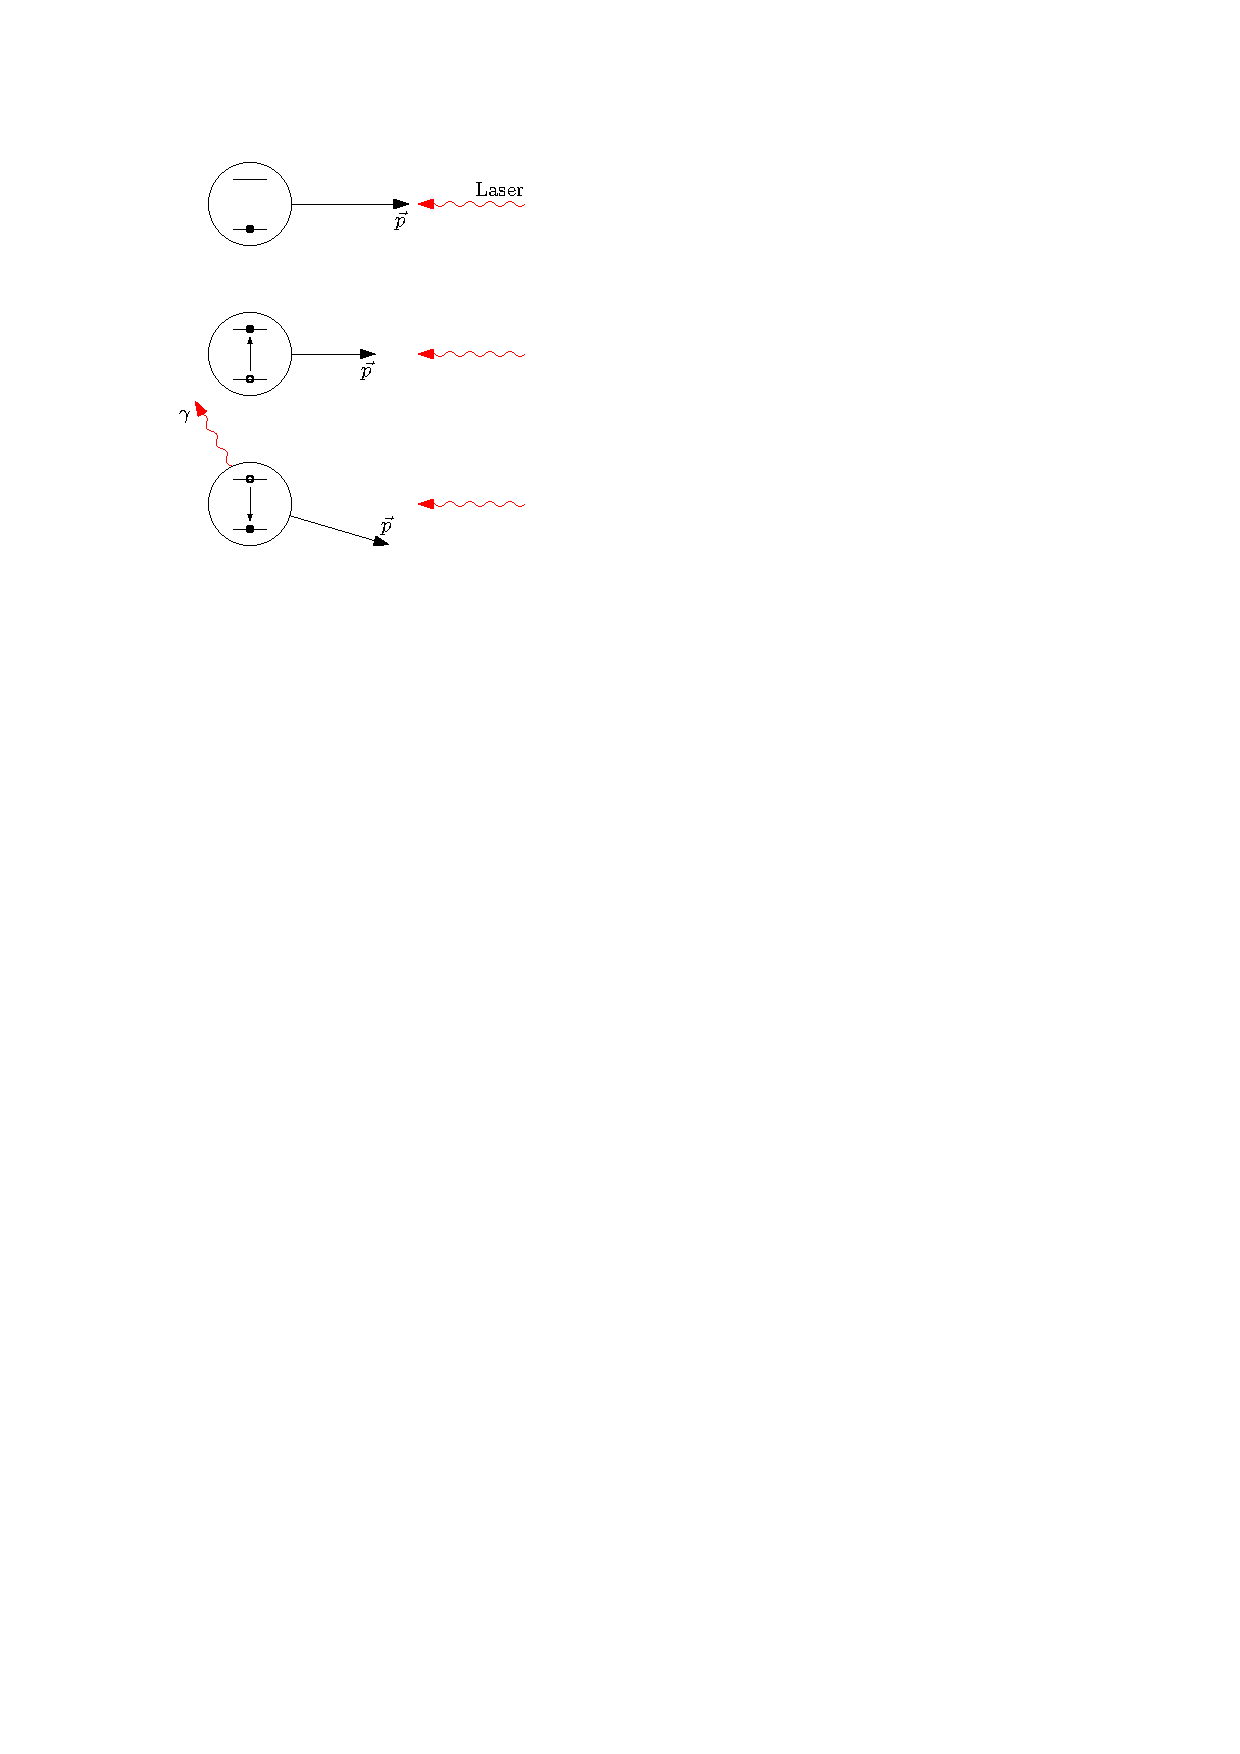
\includegraphics{./figures/theory/streukraft.pdf}
	\caption{Impulsübertrag eines Photons auf ein zu kühlendes Atom. Oben: Laserlicht wird entgegen der Flugrichtung des Atoms eingestrahlt. Mitte: durch Absorption nimmt der Impuls des Atoms ab und dieses wird angeregt. Unten: die Richtung des in Folge der Abregung emittierten Photons ist zufällig, das Atom erfährt erneut einen Impulsübertrag.}
	\label{fig:streukraft}
\end{figure}
Der mittlere Impulsübertrag bei der Emission des Photons verschwindet, da diese isotrop stattfindet.
Dennoch erfährt das Atom einen mittleren Impulsübertrag, da das Atom bei Absorption eines Photons aus einem monoenergetischen Laserstrahl stets denselben Impulsübertrag erfährt.

Ein sich bewegendes Atom nimmt aufgrund seiner Geschwindigkeit $v$ das Laserlicht wegen des Dopplereffekts mit einer um $kv$ verschobenen Frequenz gegenüber der im Laborsystem wahr.
Dies kann zur Kühlung der Atome genutzt werden, indem der Laser bezüglich des Energieabstands der beiden Niveaus, die zum Kühlen verwendet werden, rotverstimmt ist, das heißt eine geringere Frequenz hat.
Aufgrund des Dopplereffekts nimmt ein Atom, welches sich entgegen der Richtung des Laserstrahls bewegt, das Licht des Laser mit einer Frequenz wahr, welche das Atom mit einer höheren Wahrscheinlichkeit in den angeregten Zustand versetzt.
Durch die Absorption des Photons, deren Impulsübertrag immer in die gleiche Richtung zeigt und die isotrope Emission wird ein Atom, welches sich entgegen der Richtung des Laserstrahls bewegt, gebremst.
Da die Rotverschiebung geschwindigkeitsabhängig ist, ist auch die resultierende kühlende Kraft auf das Atom proportional zur Geschwindigkeit, weswegen die Kühlung auch als optische Melasse bezeichnet wird.
Unter der Verwendung von drei Paaren entgegen gerichteter Laserstrahlen die senkrecht aufeinander stehen, kann eine Kühlung von Atomen in drei Raumdimensionen durchgeführt werden.
Für ein Zweiniveausystem in einer Raumrichtung ist dies schematisch in Abbildung \ref{fig:opt_melasse} dargestellt.
\begin{figure}[h]
	\centering
	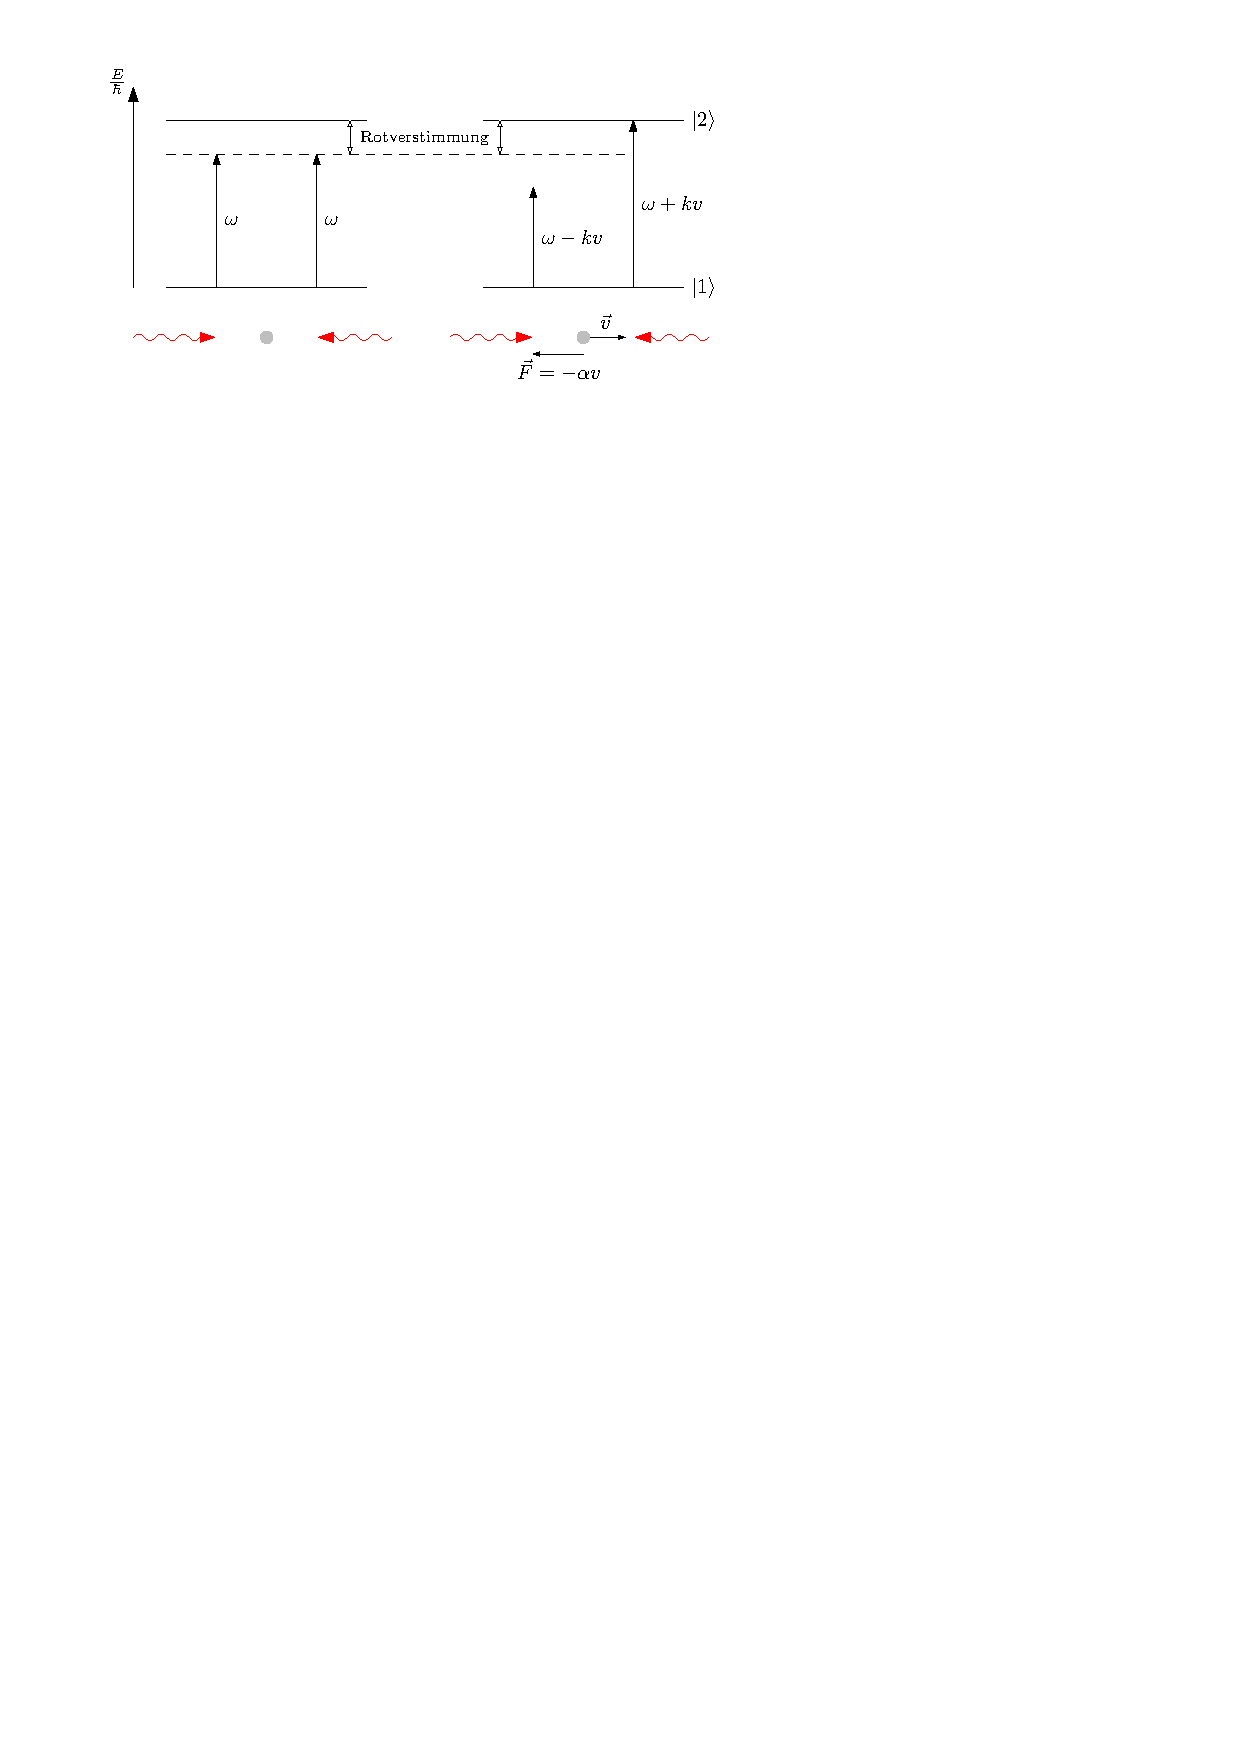
\includegraphics[width=.8\textwidth]{./figures/theory/melasse}
	\caption{Optische Melasse eines Zweiniveausystems. Links: Kraftwirkung auf ein ruhendes Atom. Rechts: der Bewegung eines Atoms entgegengesetzte Kraft.}
	\label{fig:opt_melasse}
\end{figure}

\subsection{Fangen von Atomen}
Im Folgenden wird nur ein vereinfachtes Zweiniveausystem mit~$J = 0, 1$ betrachtet, da reale Atome eine Vielzahl von Energieniveaus besitzen, die die hier durchgeführte Betrachtung deutlich verkomplizieren.
Um die gekühlten Atome, die sich zwar mit geringerer Geschwindigkeit aber weiterhin frei bewegen, an einem bestimmten Punkt zu konzentrieren wird der Zeeman-Effekt genutzt.
Dieser bewirkt eine Aufspaltung des zuvor entarteten $J=1$ Niveaus in drei Zustände mit $m_J = 0, \pm1$ durch ein externes Magnetfeld.
Die Energieverschiebung vom ursprünglichen Niveau entspricht dabei
\begin{align*}
	\Delta E =\mu_\mathrm{B} B m_J g_J
\end{align*}
mit dem Bohrschen Magneton $\mu_\mathrm{B}$, dem Landé-Faktor $g_J$, der zu dem aufgespaltenen Niveau korrespondieren Quantenzahl $m_J$ und der magnetischen Flussdichte~$B$ des externen Magnetfeldes.
Übergänge in diese Zustände können durch links- bzw. rechtszirkular polarisiertes Licht gezielt ausgewählt werden ($\sigma^\pm \leftrightarrow \Delta m_J = \pm 1$).

Für das Magnetfeld wird ein Spulenaufbau in Anti-Helmholtz-Konfiguration verwendet, der ein linear ansteigendes Magnetfeld in alle Raumrichtungen ermöglicht.
Im Zentrum des Aufbaus, in dem die Atome gefangen werden, verschwindet das Magnetfeld, nicht aber der Gradient.
Damit die Atome die Falle nicht verlassen werden, wie in Abbildung \ref{fig:magnetfeld} dargestellt, aus entgegengesetzten Richtungen jeweils ein linkszirkular und ein rechtszirkular polarisierter Laser eingestrahlt.
\begin{figure}[h]
	\centering
	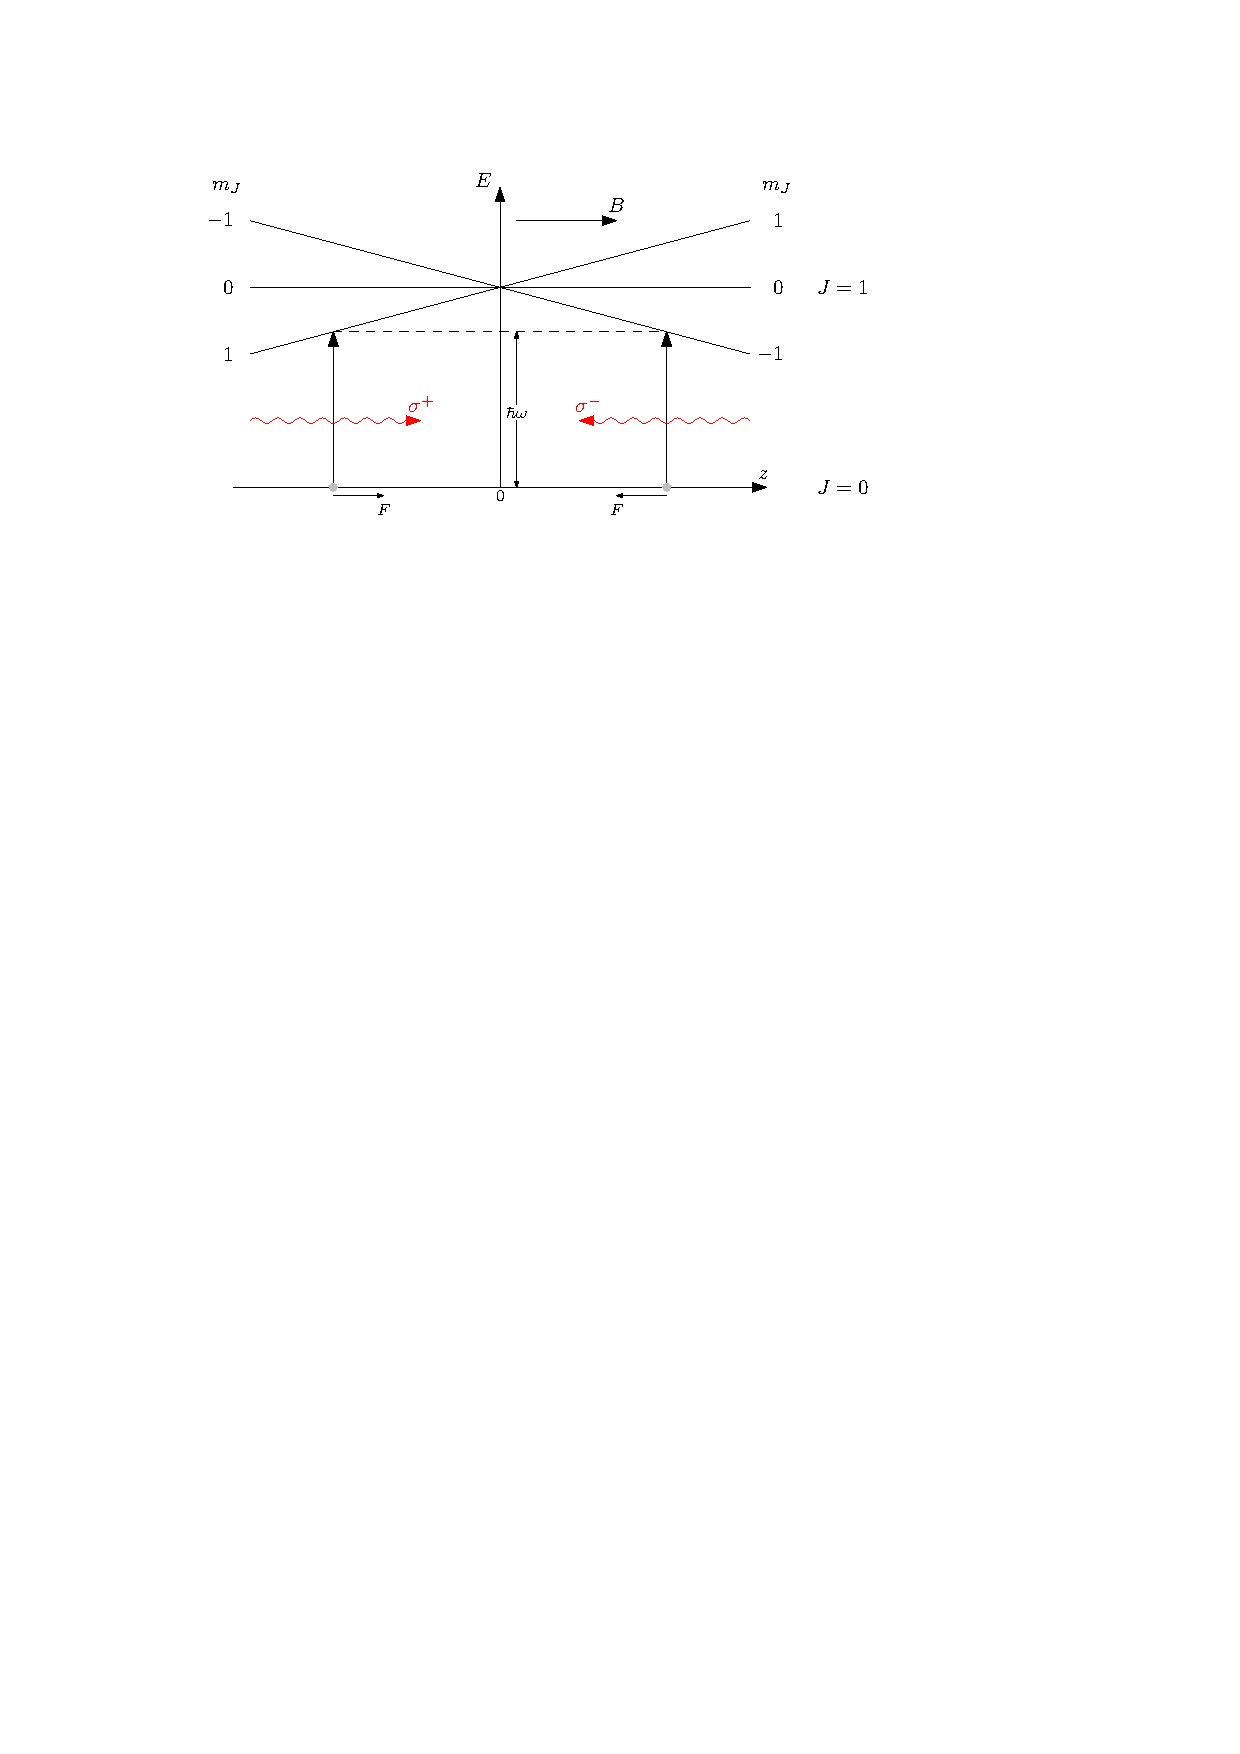
\includegraphics[width=.8\textwidth]{./figures/theory/mot.pdf}
	\caption{Ausnutzung des Zeeman-Effekts, um eine ortsabhängige Kraft auf die zu fangenden Teilchen auszuüben.}
	\label{fig:magnetfeld}
\end{figure}
Für ein nach links ausgelenktes Atom, d.h. im Bereich der Magnetfeldstärke $B<0$ liegt die Energie des Zustandes mit $m_J=+1$ unter dem Niveau mit $m_J=0$, so dass ein diesem Energieniveau gegenüber rotverstimmter Laser mit $\sigma^+$ Polarisation mit dem $m_J=+1$ Zustand wechselwirkt und eine Kraft in Richtung des Zentrum der Falle auf das Atom ausübt.
Der analoge Fall gilt für ein nach rechts ausgelenktes Atom im Bereich von $B>0$, wo der von rechts eingestrahlte Laser mit $\sigma^-$ Polarisation mit dem $m_J=-1$ Zustand interagiert, der ebenfalls unterhalb des ursprünglichen Energieniveaus liegt.
Somit erhält man durch die gezielte Einstrahlung von polarisiertem Licht, welches entsprechend dem Magnetfeld polarisiert sein muss, eine ortsabhängige Kraft auf die Atome, die sie in das Zentrum der Falle drückt und somit ein Auseinanderlaufen der gekühlten Atome verhindert.

\subsection{Übergänge in Rubidium}
\label{sec:rb_uebergaenge}

In diesem Versuch soll das Rubidiumisotop \isotope[85]{Rb} eingefangen werden.
Dazu ist es nötig, detaillierte Informationen über das Niveauschema und die Übergänge dieser Atome zu haben, um den optimalen Übergang zum Kühlen und Fangen der Atome auszuwählen.
Es eignet sich der Übergang $F=3 \rightarrow F^\prime=4$, da dieser abgeschlossen ist, d.h. dass das Atom durch Abregung vom Zustand $F^\prime=4$ ausschließlich in den Zustand $F=3$ übergeht.
Dieser Übergang entspricht einer Wellenlänge von \SI{780.25}{nm} \cite{steck}, so dass ein Laser gewählt wird, der diesem Übergang gegenüber rotverstimmt ist.
Da jedoch in einigen seltenen Fällen auch eine Anregung in die Niveaus $F^\prime=2$, $F^\prime=3$ geschieht, die in den $F=2$ Zustand übergehen können und die Atome so das abgeschlossene System zur Kühlung verlassen, wird zusätzlich ein sogenannter Pumplaser eingesetzt, der die Atome aus diesem Zustand auf das $F^\prime=2$ oder $F^\prime=3$ Niveau anhebt, von wo aus sie in das untere Niveau des Kühlübergangs mit $F=3$ zerfallen können und folglich wieder am Kühlprozess teilnehmen.
\begin{figure}[htb]
	\centering
	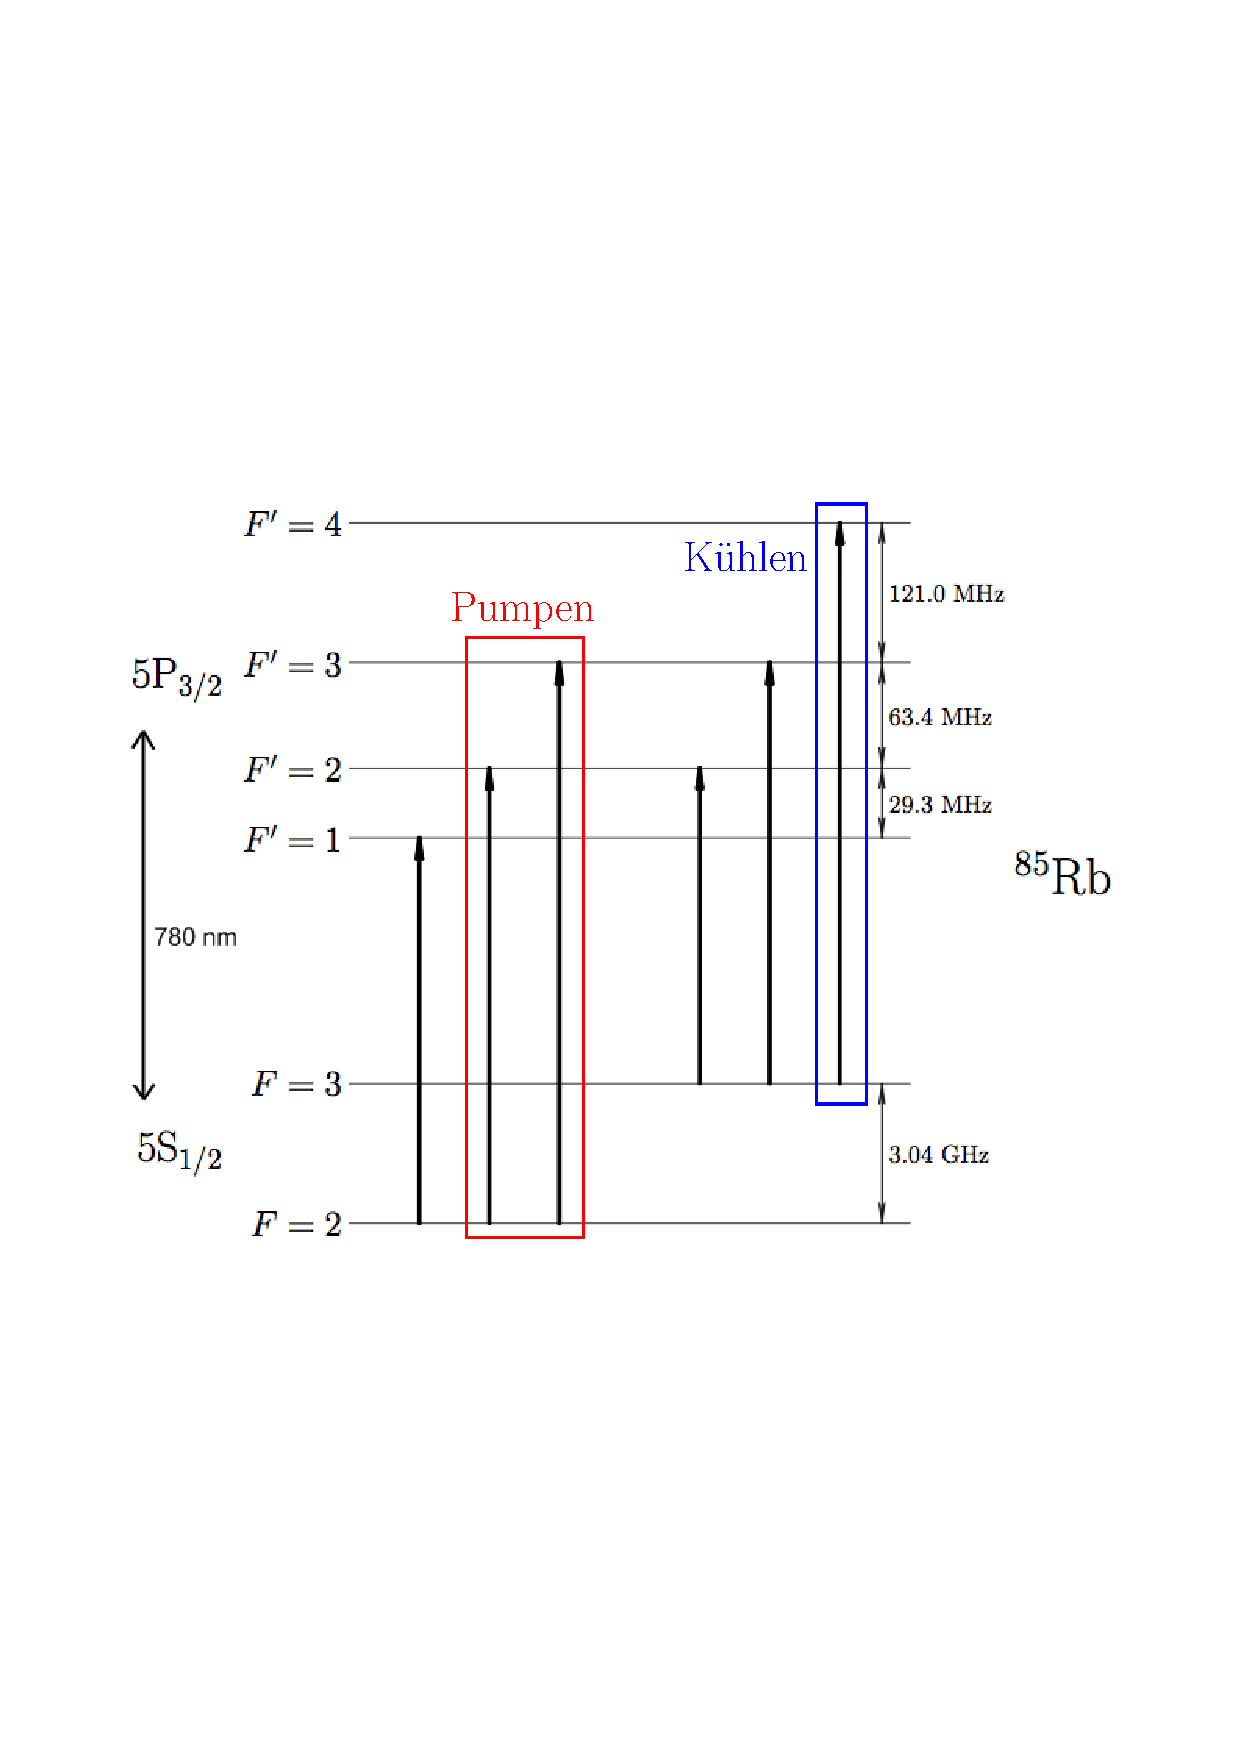
\includegraphics[width=.65\textwidth]{./figures/theory/levelscheme}
	\caption{Niveauschema von \isotope[85]{Rb} (aus \cite{script}, modifiziert).}
\end{figure}

\subsection{Lasersystem}

Wie in Abschnitt \ref{sec:rb_uebergaenge} erwähnt, werden zum Betrieb der magneto-optischen Falle zwei Laser benötigt, die auf die entsprechenden Frequenzen für den Kühl- und Pumplaser eingestellt werden müssen.
Hierzu werden zwei Diodenlaser in Littrow-Konfiguration genutzt, d.h. das emittierte Laserlicht wird kollimiert und trifft auf ein Reflexionsgitter, welches die Beugung der~-1.~Ordnung zurückreflektiert und somit einen externen Resonator bildet, während das Licht, welches in~0.~Ordnung gebeugt wird, ausgekoppelt wird, siehe Abbildung~\ref{fig:littrow}.
Durch ein elektrisch ansteuerbares Piezo-Element kann das Gitter gedreht und somit die Resonatorlänge und damit die Frequenz des ausgekoppelten Lichts geändert werden.
\begin{figure}[htb]
	\centering
	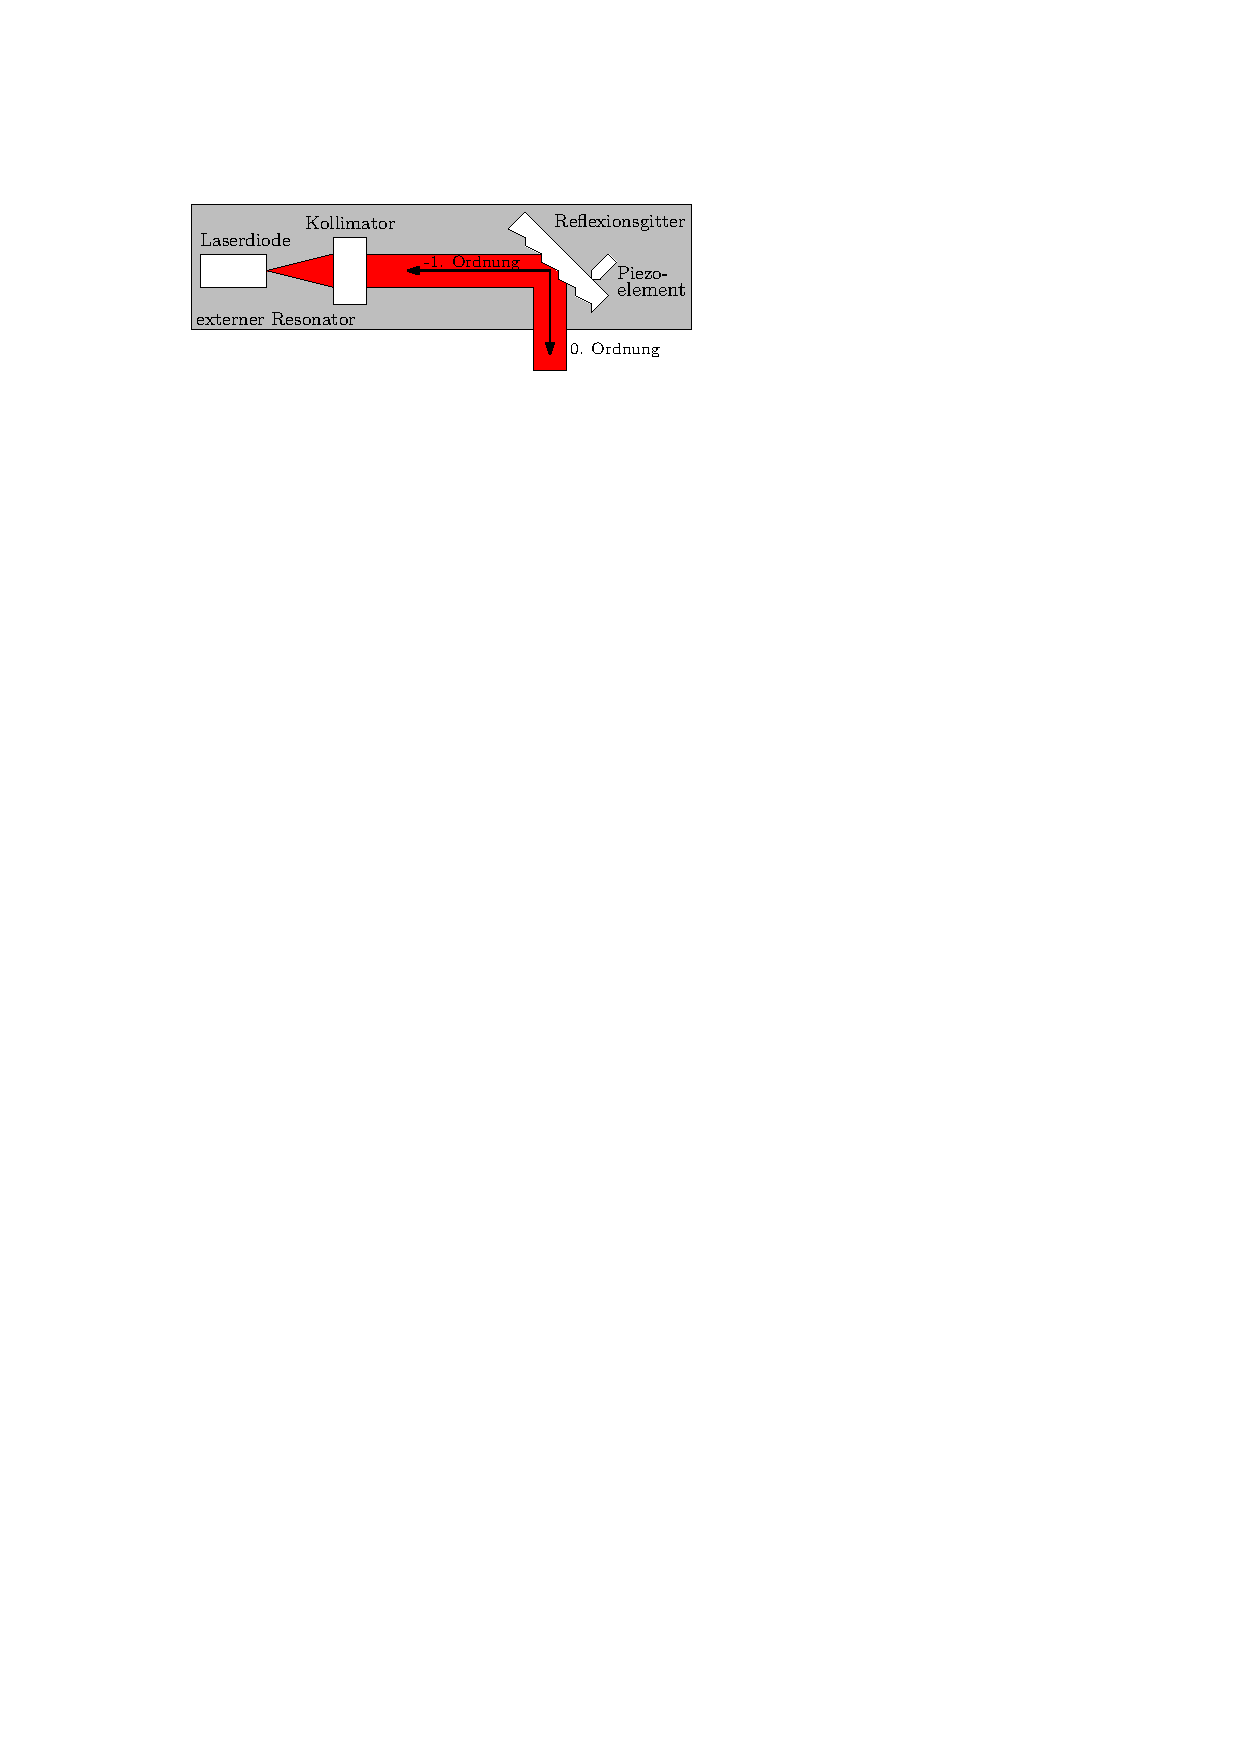
\includegraphics[width=.7\textwidth]{./figures/theory/littrow}
	\caption{Littrow-Anordnung für einen Diodenlaser. Die -1. Ordnung wird retroreflektiert, während die 0. Ordnung ausgekoppelt und für den Aufbau eines optischen Systems genutzt wird.}
	\label{fig:littrow}
\end{figure}
Da die nötigen Frequenzen möglichst genau auf die Übergänge im Rubidium abgestimmt sein müssen, wird ein Teil des Laserlichts zu Spektroskopiezwecken mit Rubidium verwendet.
Als Spektroskopieverfahren kommt die Polarisationsspektroskopie zum Einsatz, die eine Erweiterung der dopplerfreien Sättigungsspektroskopie darstellt.
Dabei wird der Lichtstrahl in einen Pumpstrahl mit hoher Intensität und einen Teststrahl mit geringerer Intensität aufgespalten, die in ungefähr entgegengesetzter Richtung eine Kammer mit Rubidiumatomen durchlaufen.
Während der Pumplaser den gewählten Übergang sättigt, d.h. möglichst viele Atome in den angeregten Zustand bringt, wird die Intensität des Teststrahls beobachtet.
Diese ist hoch, wenn der Übergang vollständig durch den Pumpstrahl gesättigt ist und gering, wenn Atome durch den Teststrahl angeregt werden.
In Abhängigkeit von der Frequenz aufgetragen ergibt sich ein Intensitätsverlauf wie in Abbildung \ref{fig:saturation}.
\begin{figure}[h]
	\centering
	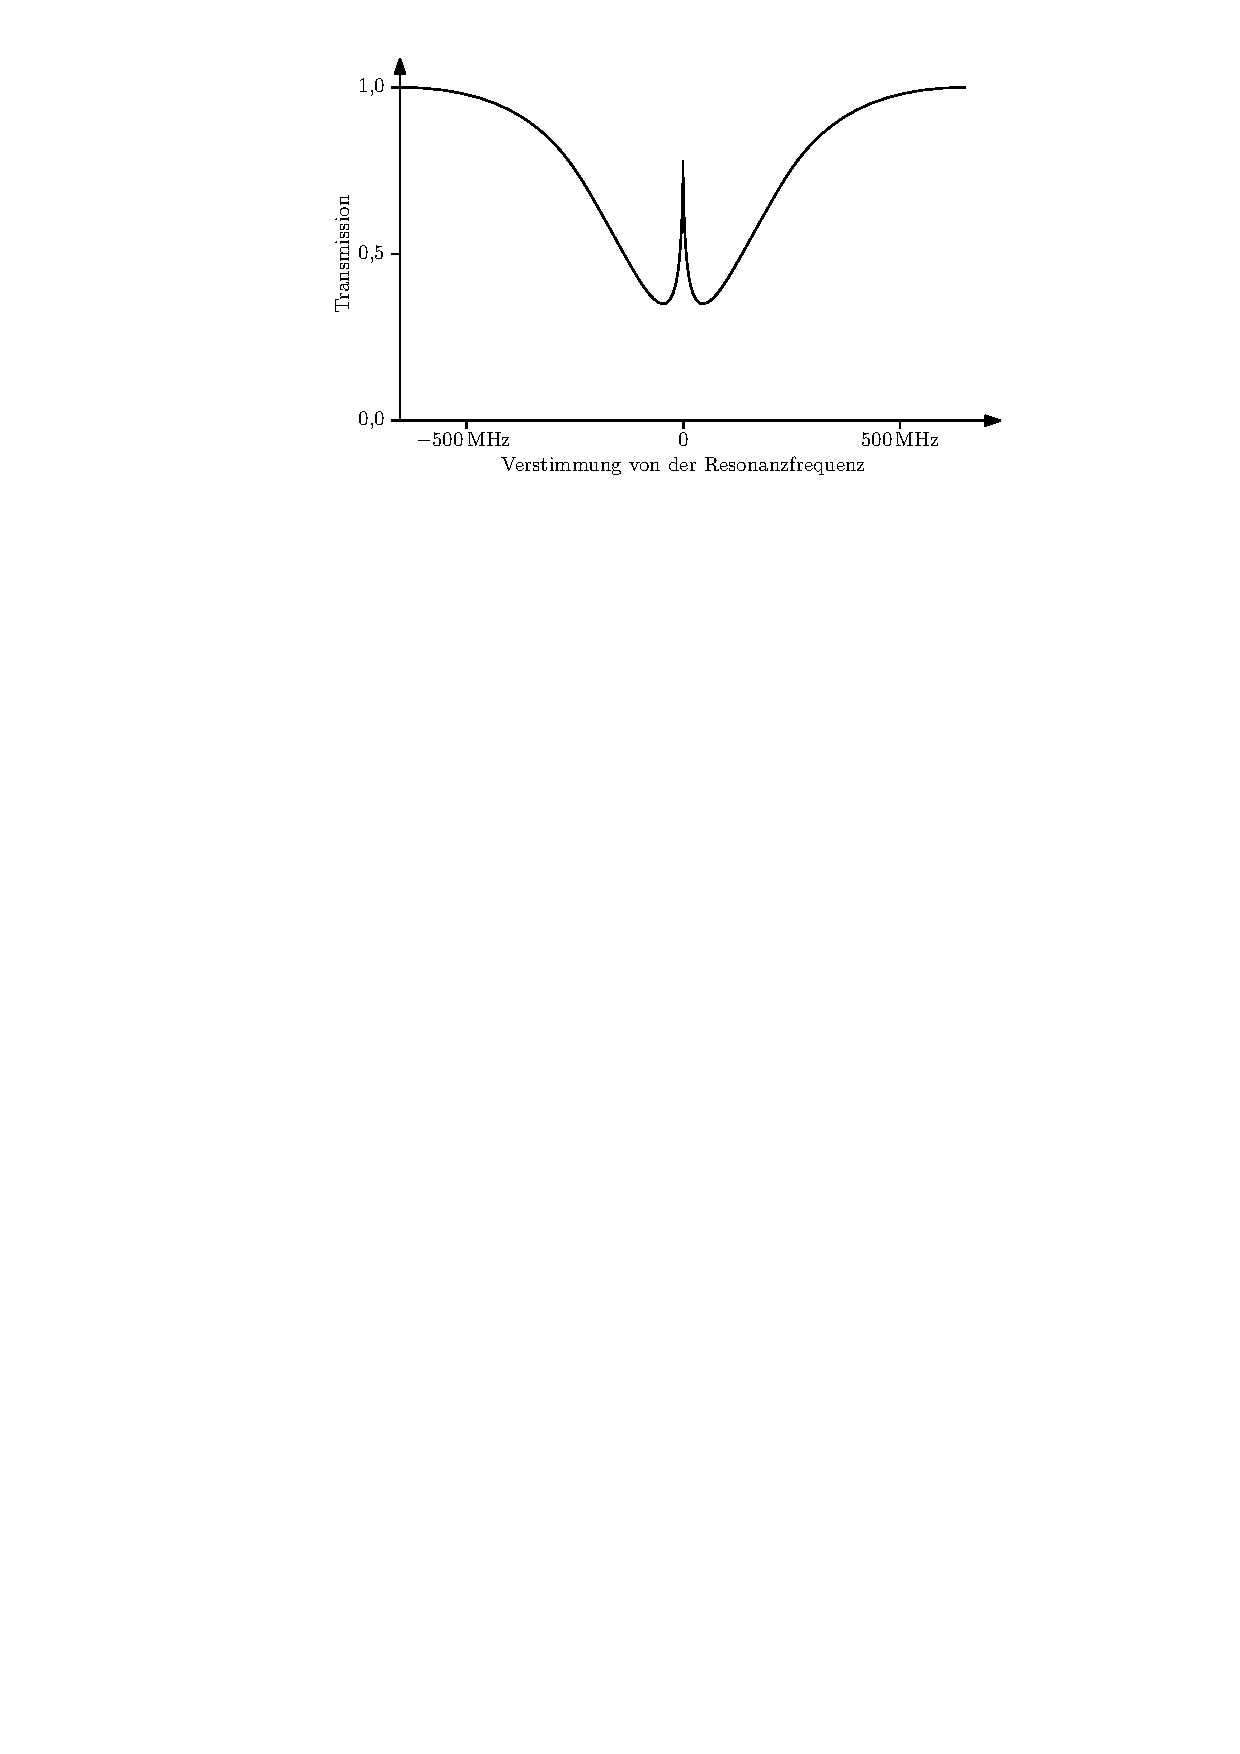
\includegraphics[width=.8\textwidth]{./figures/theory/saturation}
	\caption{Transmissionsspektrum des Teststrahls in der Sättigungsspektroskopie. Aufgrund des Dopplereffekts ist eine Senke um \SI{0}{MHz} zu beobachten, in der das dopplerfreie Maximum des betrachteten Übergangs (Lamb-Dip) liegt (nach \cite{script}).}
	\label{fig:saturation}
\end{figure}
Dieses lässt sich dadurch erklären, dass die Atome Raumtemperatur haben und sich somit sehr schnell bewegen.
Aufgrund der Dopplerverschiebung interagieren die Laser immer mit Atomen einer bestimmten Geschwindigkeitsklasse, abhängig von der Bewegungsrichtung der Atome relativ zum Laserstrahl.
Diese Bewegung ist für die Dopplerverschiebung verantwortlich und erklärt die Abflachung des Signals.
Das Maximum, auch Lamb-Dip genannt, ergibt sich durch Atome, die sich in einer Ebene senkrecht zu den Laserstrahlen bewegen.
Die Dopplerverschiebung verschwindet hier, so dass der Pumpstrahl und Teststrahl mit der gleichen Frequenz im Ruhesystems des Atoms strahlen und der Übergang somit durch den Pumpstrahl gesättigt wird, weswegen der Teststrahl keinen Intensitätsverlust erfährt.
Die natürliche Linienbreite kann auf diese Weise beobachtet werden.

In der Polarisationsspektroskopie wird der Pumpstrahl zirkularpolarisiert, so dass eines der $\Delta m_J=\pm1$ Übergänge, abhängig von der eingestrahlten Polarisation, gesättigt wird.
Diese anisotrope Besetzung ist dafür verantwortlich, dass das Rubidiumgas für die verschiedenen Zirkularpolarisationen unterschiedliche Brechungsindizes aufweist und somit das Medium optisch aktiv wird.
Dies führt dazu dass der linear polarisierte Teststrahl beim Durchgang um einen Winkel $\alpha$ gedreht wird.
Dieser Winkel ist abhängig von der Änderung des Brechungsindex für die verschiedenen Polarisationen.
Durch einen Polarisator und einen Analysator vor und hinter der Rubidiumkammer kann detektiert werden, ob die Polarisation des Teststrahls gedreht wurde.
Den Analysator bildet ein polarisierender Strahlteiler, durch den der Strahl in zwei linear polarisierte Strahlen geteilt wird, wobei beide das bekannte Spektrum der Sättigungsspektroskopie aufweisen.
Durch Subtraktion der beiden Spektren kann ein Signal generiert werden, mit dem eine Rückkopplungsschleife zur Stabilisierung der Laserfrequenz betrieben wird.
Das Signal ist hierzu besonders gut geeignet, da die Signalhöhe im Bereich um einen Übergang proportional zur Frequenzverstimmung ist.
Mithilfe einer Lockbox kann nun durch Wahl von einer Scan-Amplitude und einem Scan-Offset ein Frequenzbereich um den gewünschten Übergang eingestellt werden, um so ein Fehlersignal zu erzeugen, welches ein Piezoelement am Reflexionsgitter des Diodenlasers ansteuert.
Durch Änderung der Resonatorlänge wird somit die Frequenz des Lasers angepasst, wenn diese von der gewünschten, über die Lockbox eingestellte Frequenz, abweicht.
Dadurch ist es möglich, die Frequenz des Lasers mit hoher Genauigkeit einzustellen und Temperaturdrifts und anderen äußeren Einflüssen, die eine Änderung der Frequenz hervorrufen, entgegenzuwirken.
Darüber hinaus kann eine gewollte Verstimmung durch die das Überlagern einer konstanten Spannung erzeugt werden.

\section{Aufbau der MOT}

\subsection{Einstellung der Laserfrequenzen}

Zunächst wurden sowohl der Pump- als auch der Kühllaser auf die richtigen Frequenzen eingestellt.
Hierzu ist es wichtig, in den auf dem Oszilloskop beobachtbaren Spektren die richtigen Übergänge im Rubidium zu identifizieren, auf die die Laser eingestellt werden sollen.
Als Hilfe dienten die dargestellten Spektren in \cite{anleitung} für das \isotope[85]{Ru} Isotop.
Der Kühllaser wurde auf den Übergang $F=3 \rightarrow F^\prime=4$ eingestellt, indem durch Änderung der Scan-Amplitude und des Scan-Offsets das in der Polarisationsspektroskopie beobachtete Fehlersignal einen Nulldurchgang bei einer leichten Rotverschiebung von etwa einer halben Linienbreite gegenüber des gewünschten Rubidiumübergangs zeigt.
Durch fixieren dieses Signals mit dem Lock-Schalter an der Lockbox wird die Rückkopplungsschleife betrieben, die das Gitter am Diodenlaser ansteuert und damit die Frequenz reguliert.

Der Pumplaser wurde auf die gleiche Weise auf die Übergänge $F=2 \rightarrow F^\prime=2$ und $F=2 \rightarrow F^\prime = 3$ eingestellt, indem die Frequenzen beider Übergänge in dem durchfahrenen Frequenzbereich liegen, da der Zustand mit $F^\prime = 2$ auch zu $F=3$ zerfallen kann und so wieder dem Kühlkreislauf zugeführt wird.
Dieser Laser kann nicht über eine Rückkopplungsschleife auf eine Frequenz fixiert werden, es ist jedoch ein Betrieb der Falle  möglich, da das Signal nicht mit der gleichen Genauigkeit wie beim Kühllaser eingestellt werden muss.

\subsection{Justage der Laser an der Vakuumkammer}

Mit einem Leistungsmessgerät wurde zunächst überprüft, ob genügend Licht aus der optischen Faser austritt, wobei eine Leistung von \SI{14,5 +- 0.1}{mW} festgestellt werden konnte.
Durch zwei Strahlteiler wird das Laserlicht in drei Strahlen geteilt, die jeweils senkrecht zueinander stehen und die Vakuumkammer durchlaufen, bevor sie von einem Spiegel in sich selbst reflektiert werden, so dass insgesamt sechs Strahlen die Kammer auf drei Achsen passieren.
Zwei der Strahlen verlaufen in der horizontalen Ebene, einer entlang der vertikalen Achse.
Durch $\lambda/2$-Platten kann die Leistung der einzelnen Teilstrahlen individuell eingestellt werden, wobei alle Strahlen ungefähr die gleiche Leistung haben sollten.
Für den vertikalen Strahl wurde eine Leistung von \SI{3,0 +- 0.1}{mW} eingestellt, für die beiden horizontalen \SI{3,0 +- 0.1}{mW} bzw. \SI{3,2 +- 0.1}{mW}.
Da diese Leistungen sich nicht zu den ursprünglich zur Verfügung stehenden \SI{14,5}{mW} an der Faser addieren, kann festgestellt werden, dass in dem Aufbau eine Lichtleistung von ca. \SI{5,3}{mW} verloren geht.
Dies ist vermutlich zum Großteil auf die Verluste in den Verzögerungsplatten zurückzuführen.

Im Anschluss wurden die Aufbauten, d.h.\ die Spiegel und Einstellung der $\lambda/4$ Platten optimiert, so dass sich auf den drei Achsen sowohl einfallender als auch reflektierter Laserstrahl überlagern und sich die Strahlen im Zentrum der Vakuumkammer kreuzen.
Nach Einschalten des Magnetfeldes konnte mit der CCD-Kamera bereits eine Fluoreszenz und eine kleine Wolke gefangener Rubidiumatome erkennen.

\subsection{Optimierung der gefundenen Einstellungen}

Während eine Änderung der Rotverschiebung des Kühllasers nur eine geringe Auswirkung auf die Größe und Intensität der beobachteten Atome zeigte, konnte vor allem durch eine Feinjustage vom Frequenzbereich des Pumplaser, welcher im Scan-Modus betrieben werden musste, eine Verbesserung der Falle durchgeführt werden.
Ein zusätzliches konstantes Magnetfeld verschlechterte das beobachtete Bild, so dass diese Möglichkeit zur Optimierung nicht genutzt wurde.
Nach Anbringen eines Leistungsmessgeräts zur Bestimmung der Fluoreszenzleistung der Falle konnte auch quantitativ eine Optimierung vorgenommen werden.
So konnte eine Leistung von \SI{114 +- 5}{nW} erreicht werden, wobei dieser Wert aufgrund von Temperaturschwankungen im Raum und daher Änderungen der Laserfrequenz des nicht fixierten Pumplasers mit der Zeit eine Veränderung erfuhr.
Nachdem sich näherungsweise ein thermisches Gleichgewicht eingestellt hatte, war diese Veränderung jedoch gering, so dass die folgenden Messungen durchgeführt werden konnten, wobei gegebenenfalls zwischen zwei Messungen eine Nachjustierung des Pumplasers erfolgte.

\section{Charakterisierung der MOT}
\label{sec:charakterisierung_mot}
Nachdem die MOT aufgebaut und auf möglichst hohe Fluoreszenz optimiert wurde, kann im Folgenden die Charakterisierung einiger Eigenschaften der Falle durchgeführt werden.

\subsection{Atomzahl in der MOT}
Im Folgenden soll die Anzahl der gefangenen Atome in der MOT bestimmt werden.
Dazu muss zunächst die Fluoreszenzleistung der gefangenen Atome und der Strahlradius des Lasers bestimmt werden.

\subsubsection{Bestimmung der Fluoreszenz der MOT}
\label{sec:fluoreszenz}
Zur Bestimmung der Fluoreszenz der MOT wird die leuchtende Atomwolke mithilfe einer Linse auf ein Leistungsmessgerät abgebildet.
Dabei ist zu beachten, dass die so gemessene Leistung auch die Fluoreszenz von ungefangenen Atomen beinhaltet.
Daher wird nach jeder Messung das Magnetfeld der Falle deaktiviert, um eine Hintergrundmessung durchzuführen und der so gemessene Hintergrund kann vom Fluoreszenzsignal abgezogen werden.
Somit wird die Fluoreszenzleistung, die die Atomwolke in dem von der Linse aufgespannten Raumwinkel emittiert, zu
\begin{align*}
	P_\mathrm{Linse} = \SI{114 +- 5}{nW}
\end{align*}
bestimmt.
Um die Fluoreszenzleistung zu erhalten, die im gesamten Raumwinkel von~$4\pi$ emittiert wird, kann
\begin{align*}
	P_\mathrm{tot} = P_\mathrm{Linse} \cdot \frac{A_\mathrm{tot}}{A_\mathrm{Linse}}
\end{align*}
genutzt werden.
Dabei beschreibt $A_\mathrm{Linse}$ die Fläche der Linse und $A_\mathrm{tot}$ die Oberfläche der Kugel mit einem Radius $R$, der dem Abstand der MOT zur Linse entspricht.
Somit erhält man
\begin{align*}
	P_\mathrm{tot} = P_\mathrm{Linse} \cdot \frac{4 \pi R^2}{\frac{1}{4} \pi d_\mathrm{Linse}^2} = P_\mathrm{Linse} \cdot \frac{16 R^2}{d_\mathrm{Linse}^2}
\end{align*}
und mit den gemessenen Werten für den Linsendurchmesser
\begin{align*}
	d_\mathrm{Linse} = \SI{2.5 +- 0.1}{cm} \, \text{,}
\end{align*}
sowie dem Abstand~$R$ zwischen MOT und Linse
\begin{align*}
	R = \SI{10.3 +- 0.2}{cm}
\end{align*}
kann die gesamte Leistung berechnet werden.
Diese ergibt sich zu
\begin{align*}
	P_\mathrm{tot} = \SI{30.9 +- 3.1}{\micro\watt} \, \text{,}
\end{align*}
wobei der Fehler durch \textsc{Gauß}sche Fehlerfortpflanzung gemäß
\begin{align*}
	\Delta P_\mathrm{tot} = \frac{16}{d_\mathrm{Linse}^3} \sqrt{4 R^2 P_\mathrm{Linse}^2 d_\mathrm{Linse}^2 \Delta R^2 + R^4 \left( d_\mathrm{Linse}^2 \Delta P_\mathrm{Linse}^2 + 4 P_\mathrm{Linse}^2 \Delta d_\mathrm{Linse}^2 \right)}
\end{align*}
berechnet wurde.


\subsubsection{Bestimmung des Strahlradius}
\label{sec:strahlradius}
Anschließend muss eine Bestimmung des Radius des Laserstrahls durchgeführt werden.
Dazu wird das Leistungsmessgerät in den Strahlengang gestellt und der Laser wird seitlich durch eine Messerklinge blockiert.
Durch eine Messung der Leistung des teilweise blockierten Laserstrahls in Abhängigkeit der Position der Klinge kann der Strahlradius bestimmt werden.
Dazu wird angenommen, dass der Laserstrahl durch einen \textsc{Gauß}-Strahl beschrieben werden kann, weshalb die Intensität des Strahls in der transversalen Ebene durch
\begin{align*}
	I(x, y) = \frac{2 P_0}{\pi w^2} \exp\left(-\frac{2 (x^2 + y^2)}{w^2} \right)
\end{align*}
mit der Gesamtleistung des Strahls~$P_0$ und dem Strahlradius~$w$, das ist die Entfernung zum Strahlmittelpunkt bei dem die Intensität auf $\sfrac{1}{e^2}$ abgefallen ist, gegeben ist.
Durch Integration kann nun die Leistung des teilweise blockierten Strahls bestimmt werden
\begin{align}
	P(x) &= \int_{x}^{\infty} \mathrm{d}x^\prime \int_{-\infty}^{\infty} \mathrm{d}y^\prime \, I(x^\prime, y^\prime) \\
	     &= \frac{P_0}{2} \left[ 1 - \erf\left( \frac{\sqrt{2} x}{w}\right) \right] \, \text{,}
	\label{eq:erf_fit}
\end{align}
wobei $x$ den von der Klinge blockierten Teil des Strahls beschreibt.

\begin{figure}
	\centering
	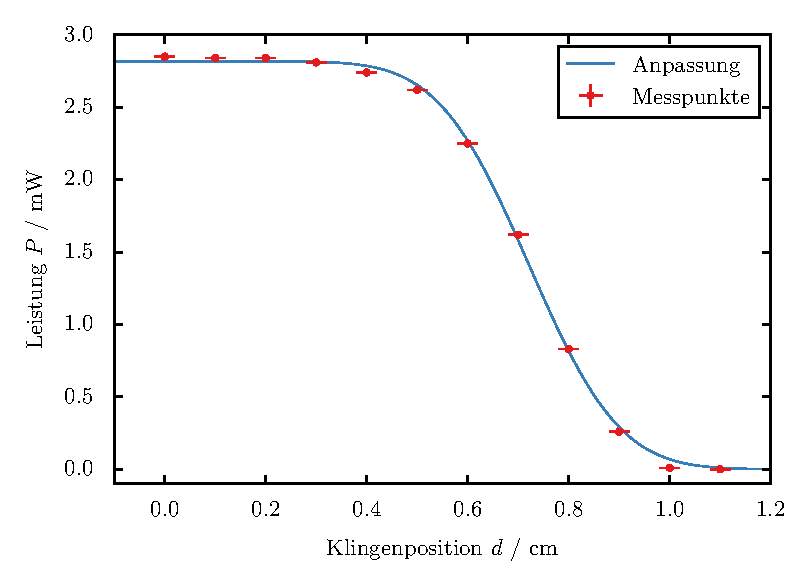
\includegraphics{./figures/beam_radius_fit.pdf}
	\caption{Anpassung einer Funktion gemäß der Hypothese in Gleichung~\eqref{eq:erf_fit} an die transmittierten Leistungen~$P$ nach der Blockierung des Strahlengangs mit einer Klinge an der Position~$x$. Der Fehler der Leistung~$\Delta P$ liegt in der Größenordnung der Markierung.}
	\label{fig:beam_radius}
	
	\vspace{1cm}
	
	\begin{tabular}{S[table-format=1.1]S[table-format=1.1]S[table-format=1.2]S[table-format=1.2]}
\toprule
{$x$ / \si{mm}} & {$\Delta x$ / \si{mm}} & {$P$ / \si{mW}} & {$\Delta P$ / \si{mW}} \\
\midrule
            0.0 &                    0.2 &            2.85 &                   0.02 \\
            1.0 &                    0.2 &            2.84 &                   0.02 \\
            2.0 &                    0.2 &            2.84 &                   0.02 \\
            3.0 &                    0.2 &            2.81 &                   0.02 \\
            4.0 &                    0.2 &            2.74 &                   0.02 \\
            5.0 &                    0.2 &            2.62 &                   0.02 \\
            6.0 &                    0.2 &            2.25 &                   0.02 \\
            7.0 &                    0.2 &            1.62 &                   0.02 \\
            8.0 &                    0.2 &            0.83 &                   0.02 \\
            9.0 &                    0.2 &            0.26 &                   0.02 \\
           10.0 &                    0.2 &            0.01 &                   0.02 \\
           11.0 &                    0.2 &            0.00 &                   0.02 \\
\bottomrule
\end{tabular}

	\captionof{table}{Transmittierte Leistung des Strahls~$P$ in Abhängigkeit der Klingenposition~$x$ zur Bestimmung des Strahlradius~$w$.}
	\label{tab:beam_radius}	
\end{figure}

Da in der Praxis keine relative Messung von Klingenposition~$x$ zum Strahlmittelpunkt durchgeführt werden kann, wird stattdessen eine Anpassung der um $\mu$ verschobenen Funktion $P(x-\mu)$ an die gemessenen Leistungen durchgeführt, um aus der Messung die Strahlleistung~$P_0$, den Strahlradius~$w$ und den Strahlmittelpunkt~$\mu$ zu extrahieren.
Die Anpassung einer solchen Kurve an die gemessenen Werte aus Tabelle~\ref{tab:beam_radius} 
führt zu den Anpassungsparametern:
\begin{align*}
	P_0 &= \SI{2.818 +- 0.017}{mW} \\
	w &= \SI{2.826 +- 0.089}{mm} \\
	\mu &= \SI{7.217 +- 0.033}{mm} \, \text{.}
\end{align*}
Die Messpunkte sowie die Anpassung wurden in Abbildung~\ref{fig:beam_radius} dargestellt.
Durch die Anpassung wurde demnach der Strahlradius~$w$ zu \SI{2.826 +- 0.089}{mm} bestimmt und kann folglich für die Auswertung verwendet werden.

\subsubsection{Streurate}
Weiterhin muss die Streurate~$R$ des Kühllasers mit einer Verstimmung~$\delta$ vom Kühlübergang mit natürlicher Linienbreite~$\Gamma$ bestimmt werden.
Diese ist gegeben durch
\begin{align*}
	R = \frac{\Gamma}{2} \frac{I / I_\mathrm{S}}{1 + I / I_\mathrm{S} + 4 \delta^2 / \Gamma^2}
\end{align*}
mit der Intensität des Lasers~$I$ und der Sättigungsintensität~$I_\mathrm{S}$ des Übergangs \cite{foot}.
Im Folgenden wird der Strahlradius~$w$, welcher in Abschnitt~\ref{sec:strahlradius} bestimmt wurde, genutzt, um die Intensität des Kühlstrahls abzuschätzen.
Dabei wird die Gesamtleistung des Kühllasers berechnet durch
\begin{align*}
	P_\mathrm{K"uhl.} &= 2 \cdot \left[ \SI{3.0 +- 0.1}{mW} + \SI{3.0 +- 0.1}{mW} + \SI{3.2 +- 0.1}{mW} \right]\\
	  &= \SI{18.4 +- 0.4}{mW} \, \text{,}
\end{align*} 
wobei der Faktor 2 aufgrund der Rückreflexion des Kühlstrahls entsteht.
Nimmt man an, dass diese Leistung gleichmäßig auf einem Kreis mit Radius~$w$ verteilt ist, so erhält man mit dem Ergebnis für den Strahlradius aus Abschnitt~\ref{sec:strahlradius} für die Intensität
\begin{align*}
	I = \frac{P_\mathrm{K"uhl.}}{\pi w^2} = \SI{73.3 +- 4.9}{\milli\watt\per\centi\meter\squared} \, \text{.}
\end{align*}
Unter der Verwendung der natürlichen Linienbreite~$\Gamma = \SI{38.117+-0.011}{MHz}$, der Sättigungsintensität~$I_\mathrm{S} = \SI{1.66932 +- 0.00052}{\milli\watt\per\centi\meter\squared}$ aus \cite{steck}, sowie der Verstimmung des Kühllasers~$\delta = \SI{-11.6+- 0.4}{MHz}$ (wird in Abschnitt~\ref{sec:detuning_cooling} bestimmt) erhält man die Streurate
\begin{align*}
	R = \SI{18.5 +- 0.1}{MHz} \, \text{.}
\end{align*}
Der Fehler wurde dabei durch \textsc{Gauß}sche Fehlerfortpflanzung berechnet.

\subsubsection{Bestimmung der Anzahl der gefangenen Atome}
\label{sec:atomzahl}
Schließlich sind alle nötigen Größen bekannt und eine Berechnung der Anzahl der gefangenen Atome kann durchgeführt werden.
Diese kann aus der gesamten Fluoreszenzleistung der gefangenen Atome~$P_\mathrm{tot}$ (Bestimmung in Abschnitt \ref{sec:fluoreszenz}), der Streurate~$R$ der Photonen des Kühllasers (Bestimmung im vorigen Abschnitt) und der bekannten Energie des Übergangs $\hbar \omega = \SI{1.589}{\electronvolt}$ \cite{steck} berechnet werden.
Somit folgt die Anzahl der gefangenen Atome
\begin{align*}
	N = \frac{P_\mathrm{tot}}{\hbar \omega R}
\end{align*}
und mit den zuvor berechneten Größen
\begin{align*}
	N = \num{6.6 +- 0.7e6} \, \text{.}
\end{align*}
Der Vergleich mit den in \cite{wieman} erreichten \num{4e7} Atomen zeigt, dass die Größenordnung der Anzahl der gefangenen Atomen übereinstimmt.
Mit zusätzlicher Feinjustage und einer funktionstüchtigen Frequenzstabilisierung für den Pumplaser sollte demnach die Größenordnung von $10^7$ Atomen mit dem vorliegenden Aufbau zu leicht erreichen sein.


\subsection{Größe der MOT}
Zur Bestimmung der Größe wird mit der CCD-Kamera ein Bild der in der Falle gefangenen Atome erstellt.
Um die Größe anzugeben, wurde im Anschluss bei gleicher Brennweite eine Millimeterskala im gleichen Abstand wie die Falle aufgenommen.
Dadurch konnte der Längenmaßstab der Aufnahmen zu~$\SI{1}{px}=\SI{0,0377+-0,0005}{mm}$ \korr{evtl.\ Bild von der Skala} bestimmt werden.
Entsprechend beträgt die Fläche eines Pixels dann~\SI{1.421+-0.038e-3}{mm^2}.
Mit einem Bildbearbeitungsprogramm wurden in dem aufgenommenen Bild mehrere Abstände gegenüberliegender Punkte auf dem Rand des markierten Bereichs gemessen, da die beobachtete Atomwolke keiner geometrischen Figur ähnelt, deren Durchmesser einfach berechnet werden könnte.
Die gemessenen Strecken wurden im Anschluss gemittelt und so der Durchmesser zu ungefähr \SI{1,47+-0,12}{mm} bestimmt, wobei der Fehler aus der Varianz folgt.
Durch eine Zählung der Pixel konnte weiterhin eine Fläche von \SI{1,16+-0,2}{mm^2} ermittelt werden.
Der Fehler wurde in diesem Fall abgeschätzt aufgrund von einer möglicherweise nicht idealen Auswahl des zu vermessenden Bereichs und entspricht einer Abweichung von~\num{162} Pixeln.
In Abbildung \ref{fig:mot_groesse} ist der untersuchte Bereich zur Bestimmung von Durchmesser und Fläche zu sehen.
\begin{figure}[h]
	\centering
	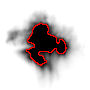
\includegraphics[width=.7\textwidth]{./figures/size_inverted.png}
	\caption{Zur Auswertung genutzter Bereich im mit der CCD-Kamera aufgenommenen Bild. Für eine bessere Druckqualität wurden die Farben invertiert.}
	\label{fig:mot_groesse}
\end{figure}

\subsection{Einfluss der $\lambda / 4$-Platten}
Im Folgenden soll der Einfluss der $\lambda / 4$-Platten auf die Population der Falle untersucht werden.
Dazu wird erneut die MOT durch eine Linse auf das Leistungsmessgerät abgebildet, um ein Fluoreszenzsignal zu messen.
Die im Aufbau genutzten $\lambda / 4$-Verzögerungsplatten lassen sich in zwei Gruppen einteilen.
Diese sind die Platten für den in die Falle eingehenden Strahl und die für den reflektierten Strahl direkt am retroreflektierenden Spiegel.
Da der Einfluss der einzelnen Platten für die jeweilige Fallenachse identisch ist, wird im Folgenden nur eine Achse detailliert untersucht.

\subsubsection{Verzögerungsplatte des eingehenden Strahls}
\label{sec:lambda_4_inc}
Zur Untersuchung des Einflusses der Verzögerungsplatte des eingehenden Strahls wird diese schrittweise gedreht und sowohl der Stellungswinkel~$\varphi$ als auch die Fluoreszenzleistung~$P$ (mit subtrahiertem Untergrund) gemessen.
Dabei wird der Stellungswinkel schrittweise von \SI{0}{\degree} bis \SI{180}{\degree} in \SI{10}{\degree}-Schritten verstellt, bis ein gesamter Winkelbereich von \SI{180}{\degree} vermessen wurde.
Die somit gemessene Fluoreszenzleistung in Abhängigkeit des Drehwinkels der Platte für den eingehenden Strahl wurde in Abbildung \ref{fig:lambda_4_inc} aufgetragen.
Die gemessenen Werte wurden in Tabelle \ref{tab:lambda_4} zusammengefasst.
\begin{figure}[h]
	\centering
	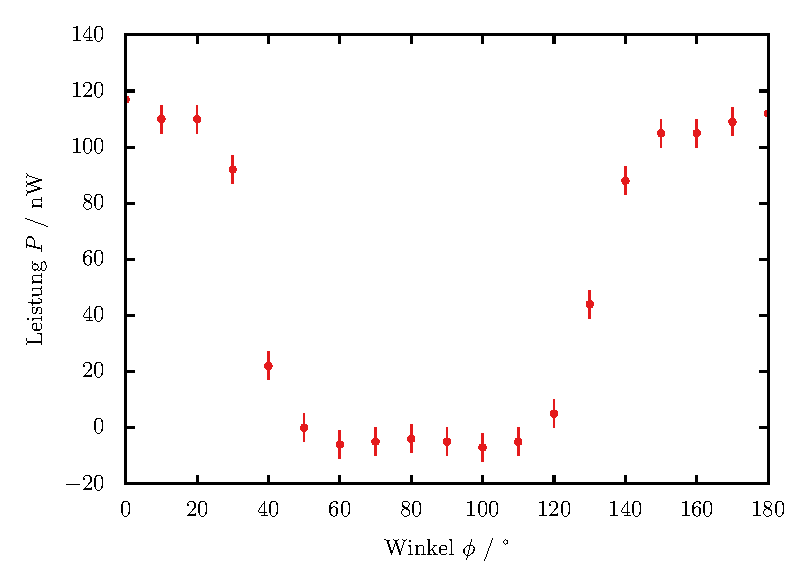
\includegraphics{./figures/lambda_4_in.pdf}
	\caption{Einfluss des Stellwinkels $\varphi$ der $\lambda / 4$-Platte des eingehenden Strahls auf die Fluoreszenz $P$ der MOT.}
	\label{fig:lambda_4_inc}
\end{figure}

Man sieht, dass die Stellung der $\lambda / 4$-Platte des eingehenden Strahls einen starken Einfluss auf die Fluoreszenzleistung zeigt.
Dies liegt daran, dass diese Platte den eintreffenden linear-polarisierten Strahl in die für die Fallenoperation notwendige zirkulare Polarisation umwandelt.
Dazu muss die Achse der Verzögerungsplatte um $\pm\SI{45}{\degree}$ gegen die Polarisation des eintreffenden Strahls verkippt sein.
Darüber hinaus muss die richtige Zirkularpolarisation für diese Platte eingestellt werden, um den gemäß Abschnitt \ref{sec:rb_uebergaenge} erforderlichen Übergang zu treffen, der eine Operation der Falle ermöglicht.

In Abbildung \ref{fig:lambda_4_inc} sieht man, dass die Fluoreszenzleistung ein breites Minimum um einen Winkel der Verzögerungsplatte von \SI{80}{\degree} aufweist.
An dieser Stelle weist der Strahl gerade die falsche Zirkularpolarisation für das Fangen der Rubidiumatome auf.
Demnach sollte ein Drehen der Verzögerungsplatte um \SI{90}{\degree} nun die entgegengesetzte Zirkularpolarisation erzeugen und somit den Fallenbetrieb ermöglichen.
Dies entspricht dem breiten Maximum bei etwa \SI{170}{\degree}, bei dem der korrekte Übergang zum Fangen der Atome angeregt wird und somit den Fallenbetrieb ermöglicht.
Der auf der Verzögerungsplatte angegebene Optimalwert von \SI{172}{\degree} kann somit verifiziert werden.

Nach dem Abschluss dieser Messung werden die drei $\lambda / 4$-Platten für die eingehenden Strahlen per Hand auf das Maximum der Fluoreszenzleistung eingestellt.
Die Vergleich der Einstellung der Platten auf den verschiedenen Achsen~$\varphi$ mit den angegebenen Optimalwerten~$\varphi^\mathrm{opt}$ zeigt eine gute Übereinstimmung:
\begin{alignat*}{2}
\varphi_x &= \SI{180}{\degree} \qquad &&\varphi_x^\mathrm{opt} = \SI{172}{\degree}\\
\varphi_y &= \SI{214}{\degree} \qquad &&\varphi_y^\mathrm{opt} = \SI{224}{\degree}\\
\varphi_z &= \SI{80}{\degree} \qquad &&\varphi_z^\mathrm{opt} = \SI{80}{\degree} \, \text{.}
\end{alignat*}


\subsubsection{Verzögerungsplatte des reflektierten Strahls}
Als nächstes soll der Einfluss der Verzögerungsplatte des reflektierten Strahls auf die Fluoreszenzleistung der MOT untersucht werden.
Dabei wird analog zu Abschnitt \ref{sec:lambda_4_inc} vorgegangen und die Fluoreszenzleistung~$P$ gegen den Winkel der Platte~$\varphi$ aufgetragen.
Die gemessenen Werte finden sich in Tabelle \ref{tab:lambda_4} und die Darstellung der Fluoreszenzleistung in Abbildung \ref{fig:lambda_4_out}.
\begin{figure}[h]
	\centering
	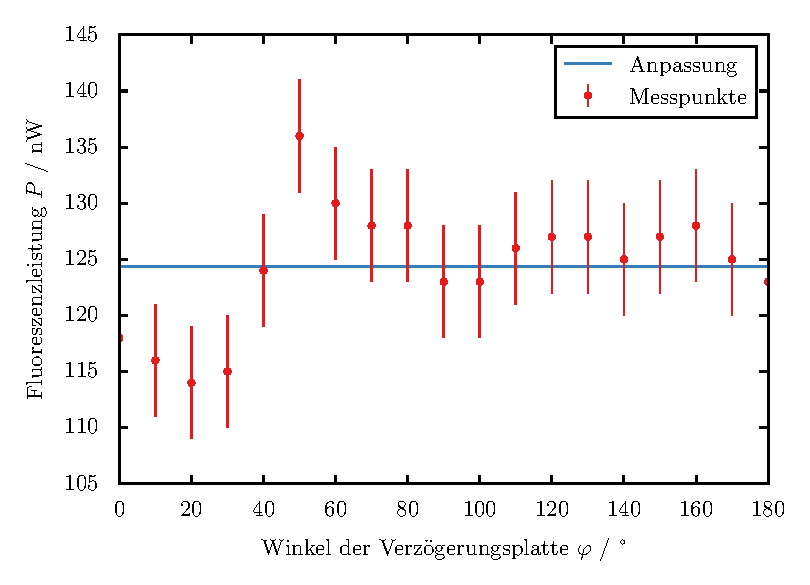
\includegraphics{./figures/lambda_4_out.pdf}
	\caption{Einfluss des Stellwinkels $\varphi$ der $\lambda / 4$-Platte des reflektierten Strahls auf die Fluoreszenz $P$ der MOT. Die Anpassung einer konstanten Funktion ergibt für die Fluoreszenzleistung $P_0 = \SI{124.4 +- 1.3}{nW}$.}
	\label{fig:lambda_4_out}
\end{figure}

Man sieht, dass die Fluoreszenzleistung kaum vom Winkel der Verzögerungsplatte abhängt.
Der Grund liegt darin, dass beim Eintreffen des zirkular-polarisierten Strahls aus dem Fallenzentrum auf die $\lambda / 4$-Platte dieser linear polarisiert wird.
Anschließend wird der linear-polarisierte Strahl am Spiegel reflektiert und trifft unter dem gleichen Winkel erneut auf die $\lambda / 4$-Platte und ist somit unabhängig von deren Stellwinkel.
Dies hat den Einfluss, dass die Helizität der Photonen umgekehrt wird und somit aus dem eingehenden Strahl mit $\sigma^\pm$-Polarisation ein rückläufiger Strahl mit $\sigma^\mp$-Polarisation entsteht.

Die Anpassung einer konstanten Funktion an die gemessene Fluoreszenzleistung ergibt
\begin{align*}
P_0 = \SI{124.4 +- 1.3}{nW}
\end{align*}
für die Fluoreszenzleistung der MOT.

\begin{table}
	\centering
	\begin{tabular}{S[table-format=3.0]S[table-format=3.0]S[table-format=3.0]}
\toprule
{$\varphi$ / \si{\degree}} & {$P_\mathrm{ein.}$ / \si{nW}} & {$P_\mathrm{ref.}$ / \si{nW}} \\
\midrule
                         0 &                           122 &                           118 \\
                        10 &                           115 &                           116 \\
                        20 &                           115 &                           114 \\
                        30 &                            97 &                           115 \\
                        40 &                            27 &                           124 \\
                        50 &                             5 &                           136 \\
                        60 &                            -1 &                           130 \\
                        70 &                             0 &                           128 \\
                        80 &                             1 &                           128 \\
                        90 &                             0 &                           123 \\
                       100 &                            -2 &                           123 \\
                       110 &                             0 &                           126 \\
                       120 &                            10 &                           127 \\
                       130 &                            49 &                           127 \\
                       140 &                            93 &                           125 \\
                       150 &                           110 &                           127 \\
                       160 &                           110 &                           128 \\
                       170 &                           114 &                           125 \\
                       180 &                           117 &                           123 \\
\bottomrule
\end{tabular}

	\caption{Gemessene Fluoreszenz der gefangenen Atome für verschiedene Stellungen der $\lambda / 4$-Platte des eingehenden Strahls~$P_\mathrm{ein.}$ und des reflektierten Strahls~$P_\mathrm{ref.}$. Auf die Fluoreszenzleistung wird ein Fehler von $\Delta P = \SI{5}{nW}$ angenommen.}
	\label{tab:lambda_4}
\end{table}


\subsection{Einfluss des Magnetfeldes}
Anschließend findet eine Messung der Fluoreszenzleistung der gefangenen Atome in Abhängigkeit des Stroms durch das Anti-Helmholtz-Spulenpaar statt.
Dieser Strom ist proportional zum Magnetfeldgradienten am Ort der Falle und hat somit einen Einfluss auf die Tiefe des Fallenpotentials.
Die gemessenen Werte der Fluoreszenzleistung~$P$ wurden in Abbildung~\ref{fig:magnetic_field} gegen den Spulenstrom~$I$ aufgetragen.
Darüber hinaus finden sich die gemessenen Werte in Tabelle~\ref{tab:magnetic_field}.
\begin{figure}[hp]
	\centering
	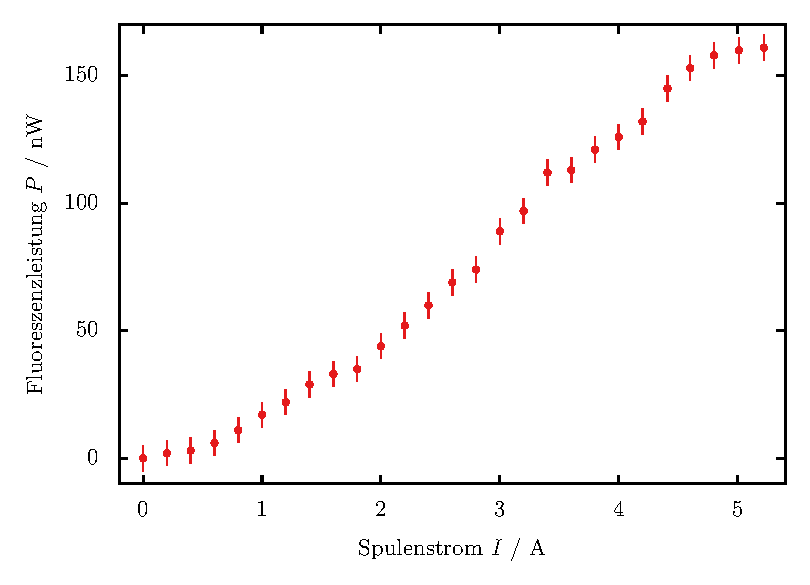
\includegraphics{./figures/magnetic_field.pdf}
	\caption{Einfluss des Spulenstroms des Anti-Helmholtz-Spulenpaares und somit des Magnetfeldgradienten im Zentrum der Falle auf die Fluoreszenzleistung der in der MOT gefangenen Atome.}
	\label{fig:magnetic_field}
	\vspace{1cm}
	\begin{minipage}[t]{0.3\textwidth}
		\centering
		\vspace*{-\dimexpr\baselineskip+\heavyrulewidth+\abovetopsep\relax}
		\begin{tabular}{S[table-format=1.2]S[table-format=3.0]}
\toprule
{Strom $I$ / \si{A}} & {Leistung $P$ / \si{nW}} \\
\midrule
                5.22 &                      161 \\
                5.01 &                      160 \\
                4.80 &                      158 \\
                4.60 &                      153 \\
                4.41 &                      145 \\
                4.20 &                      132 \\
                4.00 &                      126 \\
                3.80 &                      121 \\
                3.60 &                      113 \\
                3.40 &                      112 \\
                3.20 &                       97 \\
                3.00 &                       89 \\
                2.80 &                       74 \\
                2.60 &                       69 \\
\bottomrule
\end{tabular}

	\end{minipage} 
	\begin{minipage}[t]{0.3\textwidth}
		\centering
		\vspace*{-\dimexpr\baselineskip+\heavyrulewidth+\abovetopsep\relax}
		\begin{tabular}{S[table-format=1.2]S[table-format=3.0]}
\toprule
{Strom $I$ / \si{A}} & {Leistung $P$ / \si{nW}} \\
\midrule
                2.40 &                       60 \\
                2.20 &                       52 \\
                2.00 &                       44 \\
                1.80 &                       35 \\
                1.60 &                       33 \\
                1.40 &                       29 \\
                1.20 &                       22 \\
                1.00 &                       17 \\
                0.80 &                       11 \\
                0.60 &                        6 \\
                0.40 &                        3 \\
                0.20 &                        2 \\
                0.00 &                        0 \\
\bottomrule
\end{tabular}

	\end{minipage}
	\captionof{table}{Messwerte zur Bestimmung des Einflusses des Spulenstroms~$I$ mit einem Fehler von $\Delta I = \SI{0.01}{\ampere}$ auf die Fluoreszenzleistung der gefangenen Atome $P$ mit $\Delta P = \SI{5}{nW}$.}
	\label{tab:magnetic_field}
\end{figure}

Die Abbildung kann im wesentlichen in drei unterschiedliche Bereiche eingeteilt werden.
Zum einen ist dies der Bereich kleiner Ströme von \num{0} bis etwa \SI{1}{\ampere}, bei denen nur eine kleine Fluoreszenzleistung beobachtet werden kann, die nur langsam mit dem Spulenstrom ansteigt.
In diesem Strombereich ist der Potentialtopf zu klein um eine signifikante Anzahl von Atomen einzufangen.
Ab einem Strom von \SI{1}{\ampere} steigt die Fluoreszenzleistung stark mit dem Spulenstrom und die gefangenen Atome sind mithilfe einer Kamera klar zu erkennen.
An diesem Punkt können die Rubidiumatome effizient durch das Fallenpotential gefangen werden.
Übersteigt der Spulenstrom \SI{4.4}{\ampere} so stellt man fest, dass die Falle scheinbar in Sättigung übergeht.
\korr{Argument für die Sättigung}
Darüber hinaus finden sich einige Sprünge in den Messdaten deren Ursache bei dem Laser für das optische Pumpen der Rubidiumatome auf den Kühlübergang zu suchen sind.
Dieser kann aufgrund eines schlechten Fehlersignals nicht durch die Lockbox auf den Übergang festgestellt werden und somit leichte Abweichungen während der Messung verursachen.


\subsection{Verhalten des Ladevorgangs}
Folglich soll das Verhalten des Ladevorgangs der Atomfalle untersucht werden.
Nun werden die gefangenen Atome durch eine Linse auf eine Photodiode abgebildet, welche eine zur Fluoreszenz der gefangenen Atome proportionale Spannung erzeugt, die mit einem Oszilloskop gemessen werden kann.
Um einen Ladevorgang der Falle zu starten wird zunächst der Spulenstrom durch das Anti-Helmholtz-Spulenpaar deaktiviert sodass keine MOT mehr zu beobachten ist.
Danach wird das Magnetfeld reaktiviert und auf dem Oszilloskop kann ein exponentieller Anstieg der Fluoreszenz der gefangenen Atome beobachtet werden.
Dieser Anstieg verhält sich wie die Aufladung eines Kondensators und folglich wird die Anpassungshypothese
\begin{align}
	U(t) =  U_0 \left[ 1 - \exp\left( - \frac{t - t_0}{\tau} \right) \right] \cdot \Theta(t - t_0) + \mathrm{BG}
	\label{eq:loading_fit}
\end{align}
mit dem maximalen Fluoreszenzsignal~$U_0$ der Photodiode, der Zeitkonstante der Aufladung~$\tau$, dem Beginn des Ladevorgangs~$t_0$, der Heaviside-Funktion~$\Theta$ und einem konstanten Untergrund~$\mathrm{BG}$ verwendet.
In Abbildung \ref{fig:loading} wurde beispielhaft eine Anpassung an die Ladekurve durchgeführt.
Insgesamt wurden 11 Ladekurven zur Bestimmung der mittleren Zeitkonstante~$\bar{\tau}$ vermessen und die resultierenden Anpassungsparameter wurden in Tabelle~\ref{tab:loading_params} zusammengefasst.
\begin{figure}[htbp]
	\centering
	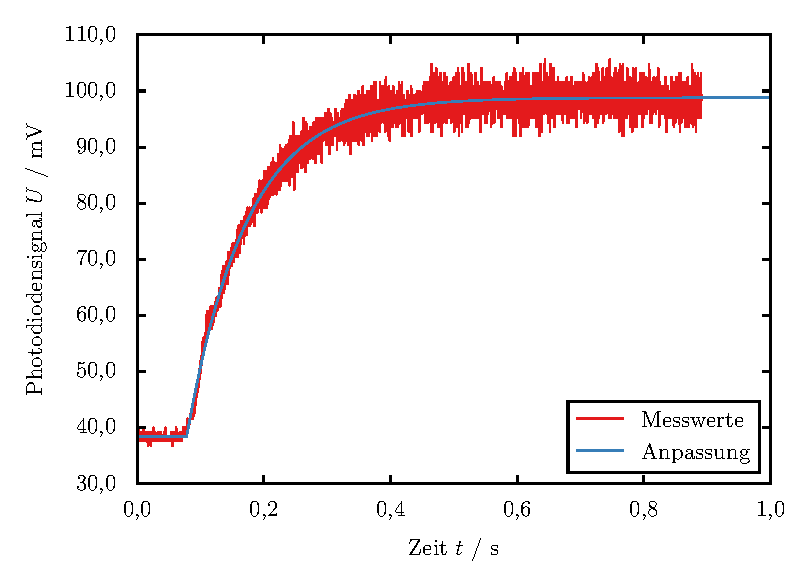
\includegraphics{./figures/loading/loading11.pdf}
	\caption{Anpassung einer Ladekurve gemäß der Anpassungshypothese in Gleichung \eqref{eq:loading_fit} an den zeitlichen Verlauf des Photodiodensignal~$U$ während des Ladevorgangs der MOT.}
	\label{fig:loading}
	
	\vspace{1cm}
	
	\resizebox{\textwidth}{!}{
		\begin{tabular}{S[table-format=2.2]S[table-format=1.2]S[table-format=3.2]S[table-format=1.2]S[table-format=3.2]S[table-format=1.2]S[table-format=2.2]S[table-format=1.2]}
\toprule
{$U_0$ / \si{mV}} & {$\Delta U_0$ / \si{mV}} & {$\tau$ / \si{ms}} & {$\Delta \tau$ / \si{ms}} & {$t_0$ / \si{ms}} & {$\Delta t_0$ / \si{ms}} & {$\mathrm{BG}$ / \si{mV}} & {$\Delta \mathrm{BG}$ / \si{mV}} \\
\midrule
            52.29 &                     0.22 &             105.09 &                      0.97 &             48.99 &                     0.71 &                     26.82 &                             0.20 \\
            52.52 &                     0.16 &             110.03 &                      0.94 &             80.53 &                     0.63 &                     27.07 &                             0.15 \\
            57.32 &                     0.17 &              97.52 &                      0.96 &            133.15 &                     0.62 &                     36.64 &                             0.14 \\
            55.88 &                     0.20 &              95.77 &                      0.95 &             86.37 &                     0.65 &                     37.41 &                             0.18 \\
            55.92 &                     0.22 &              99.23 &                      1.04 &            100.50 &                     0.72 &                     37.79 &                             0.20 \\
            50.23 &                     0.17 &              98.55 &                      1.17 &            141.01 &                     0.75 &                     38.57 &                             0.15 \\
            45.85 &                     0.27 &             103.74 &                      1.34 &             45.97 &                     0.99 &                     38.30 &                             0.26 \\
            35.51 &                     0.19 &             100.33 &                      1.64 &            109.21 &                     1.08 &                     35.35 &                             0.17 \\
            59.11 &                     0.16 &              96.21 &                      0.80 &             95.11 &                     0.53 &                     39.52 &                             0.14 \\
            56.95 &                     0.24 &              95.02 &                      0.95 &            126.57 &                     0.69 &                     38.20 &                             0.23 \\
            60.40 &                     0.19 &              94.33 &                      0.82 &             78.27 &                     0.57 &                     38.40 &                             0.17 \\
\bottomrule
\end{tabular}

	}
	\captionof{table}{Ergebnisse der Anpassungen gemäß Gleichung \eqref{eq:loading_fit} an die vermessenen Ladekurven der MOT.}
	\label{tab:loading_params}
\end{figure}

Schließlich kann aus den 11 vermessenen Ladekurven die mittlere Zeitkonstante~$\bar{\tau}$ des Aufladeprozesses bestimmt werden.
Diese beträgt
\begin{align*}
	\bar{\tau} = \SI{99.6 +- 4.9}{ms} \, \text{,}
\end{align*}
wobei der Fehler aus der Stichprobenvarianz abgeschätzt wird.

\subsubsection{Bestimmung des Rb-Rb Wirkungsquerschnittes}
Anschließend kann die Messung der mittleren Zeitkonstante~$\bar{\tau}$ dazu genutzt werden den Wirkungsquerschnitt von Rb-Rb Kollisionen zu berechnen.
Dies ist möglich, da gemäß \cite{wieman} die Zeitkonstante des Aufladeprozesses ebenfalls der mittleren Zeit entspricht, die ein Rubidiumatom in der Falle gefangen bleibt.
Demnach kann die Zeitkonstante unter Vernachlässigung weiterer Spurengase durch 
\begin{align*}
	\frac{1}{\tau} = n_\mathrm{Rb}  \sigma_\mathrm{Rb}  v_\mathrm{Rb}
\end{align*}
beschrieben werden \cite{wieman}, wobei die Rubidiumdichte~$n_\mathrm{Rb}$, der Rb-Rb Wirkungsquerschnitt~$\sigma_\mathrm{Rb}$ und die mittlere Geschwindigkeit der Rubidiumatome~$v_\mathrm{Rb}$ gegeben ist.
Somit kann der Wirkungsquerschnitt durch
\begin{align}
	\sigma_\mathrm{Rb} = \frac{1}{\tau n_\mathrm{Rb} v_\mathrm{Rb}}
	\label{eq:cross_sec}
\end{align}
berechnet werden.
Dazu wird zunächst die Rubidiumdichte~$n_\mathrm{Rb}$ benötigt, welche aus dem Druck in der Vakuumkammer~$p$ und der Temperatur~$T$ des Gases mithilfe der idealen Gasgleichung berechnet werden kann.
Dabei wurde die Temperatur~$T$ mithilfe eines Thermometers zu $\SI{24.6 +- 0.5}{\degreeCelsius}$ bestimmt.
Der Druck~$p$ in der Vakuumkammer muss auf $\SI{1.1 +- 0.2e-7}{mbar}$ abgeschätzt werden, da ein Fehler an der Druckanzeige der Vakuumpumpe vorlag.
Dann kann gemäß der idealen Gasgleichung die Rubidiumdichte durch
\begin{align*}
	n_\mathrm{Rb} = \frac{p}{k_\mathrm{B} T}
\end{align*}
bestimmt werden.
Unter Verwendung des abgeschätzten Drucks und der Temperatur des Gases erhält man
\begin{align*}
	n_\mathrm{Rb} = \SI{2.68 +- 0.49e15}{\per\meter\cubed} \, \text{,}
\end{align*}
wobei der Fehler durch \textsc{Gauß}sche Fehlerfortpflanzung berechnet wurde.
Anschließend kann mithilfe der Maxwell-Boltzmann-Verteilung die mittlere Geschwindigkeit der Rubidiumatome~$v_\mathrm{Rb}$ durch
\begin{align*}
	v_\mathrm{Rb} = \sqrt{\frac{8 k_\mathrm{B} T}{\pi m_\mathrm{Rb}}} 
\end{align*}
berechnet werden.
Mit der gemessenen Temperatur des Gases und der Masse von \isotope[85]{Rb}~$m_\mathrm{Rb} = \SI{1.41e-25}{kg}$ \cite{handbook_spectroscopic_data} erhält man
\begin{align*}
	v_\mathrm{Rb} = \SI{272.5 +- 0.3}{\meter\per\second} \, \text{.}
\end{align*}
Schließlich können diese Werte und die im vorigen Abschnitt vermessene mittlere Zeitkonstante in Gleichung \eqref{eq:cross_sec} eingesetzt werden um
\begin{align*}
	\sigma_\mathrm{Rb} &= \SI{1.37 +- 0.26e-13}{\centi\meter\squared}\\
\end{align*}
zu erhalten.

Eine Abschätzung für den tatsächlichen Wert des Rb-Rb Wirkungsquerschnittes kann aus den Ergebnissen von \cite{force_in_mot} erfolgen.
Die Interaktion der Rubidiumatome erfolgt durch resonante Dipol-Dipol-Wechselwirkung und der Wirkungsquerschnitt liegt dann in der Größenordnung von etwa~$10^{-13} \, \si{\centi\meter\squared}$.
Der in diesem Versuch bestimmte Wert fällt ebenfalls in diesen Bereich, sollte jedoch nur als grobe Abschätzung angesehen werden, da der genaue Druck in der Vakuumkammer nicht bekannt ist.


\subsection{Verstimmung der Laserfrequenzen}
Letztlich soll die Fluoreszenz der magneto-optischen Falle in Abhängigkeit der Frequenz von Kühllaser sowie Pumplaser untersucht werden.
Dazu wird jeweils einer der Laser mithilfe der Lockbox auf eine bestimmte Frequenz festgelegt, während der andere im Scan-Modus mit einer Frequenz von \SI{20}{mHz} betrieben wird.
Dadurch wird die Frequenz des Lasers in Abhängigkeit von Scan-Offset und Amplitude über einen kleinen Bereich variiert und mithilfe einer Photodiode kann die Fluoreszenz der MOT gemessen werden.
Dabei ist es wichtig die Scan-Frequenz so klein zu wählen, dass die Periode des Scan-Signals wesentlich kleiner ist als die typische Ladezeit der MOT von etwa \SI{0.1}{s}.
Darüber hinaus wird eine Untergrundmessung mit deaktiviertem Magnetfeld durchgeführt, um die Fluoreszenz des heißen Hintergrundgases entfernen zu können.
Dieser Untergrund kann mithilfe des Spektrums aus der Rb-Spektroskopie an das Fluoreszenzsignal der MOT angepasst und folglich abgezogen werden.

\subsubsection{Variation der Kühllaserfrequenz}
\label{sec:detuning_cooling}
Zunächst wird die Frequenz des Pumplasers fixiert, indem die Scan-Amplitude minimiert und mithilfe des Scan-Offset der Pumpübergang auf Resonanz gestellt wird.
Im Gegensatz zum Kühllaser konnte der Pumplaser aufgrund eines stark Verrauschten Fehlersignals nicht mithilfe der Rückkopplungsschleife fixiert werden.
Anschließend wird der Scan-Bereich des Kühllasers auf die Umgebung des Kühlübergangs eingestellt und mithilfe des Oszilloskops kann sowohl die Rb-Spektroskopie als auch das Fluoreszenzsignal der Photodiode dargestellt werden.
Nun kann die Fluoreszenz der MOT in Abhängigkeit der Verstimmung des Kühllasers gemessen werden.
Dazu wird jeweils eine Messung mit und eine ohne Magnetfeld durchgeführt, um die Hintergrundfluoreszenz in der Analyse entfernen zu können.

In Abbildung~\ref{fig:detuning_cooling} wurde sowohl das Rb-Spektrum, als auch das Fluoreszenzsignal der MOT und dessen Untergrund dargestellt.
Weiterhin wurde das Signal nach Subtraktion des Untergrundes dargestellt.
An das Signal der Rb-Spektroskopie wurde folglich eine Kurve bestehend aus drei Lorentz-Kurven und einem polynomialen Untergrund 4.\ Ordnung angepasst.
Dies ermöglicht die Bestimmung der Frequenzen der Linien im Spektrum und wurde genutzt um das Untergrundsignal an das Fluoreszenzsignal der MOT anzupassen und folglich von diesem abzuziehen.
Darüber hinaus können die bekannten Frequenzen der Linien genutzt werden um eine Frequenzeichung durchzuführen.
Dazu nutzt man die Verstimmung der beiden Überkreuzungs-Signale (im Spektrum links) gegenüber dem Kühlübergang, welche in \cite{script} gegeben ist durch $\delta_{3 \rightarrow 2,4} = \SI{-92.0}{MHz}$ ($F=3 \rightarrow F^\prime=2,4$) und $\delta_{3 \rightarrow 3, 4} = \SI{-60.3}{MHz}$ ($F=3 \rightarrow F^\prime=3,4$).
Schließlich wird an das Fluoreszenzsignal, welches bereits vom Untergrund bereinigt wurde, eine Gauß-Funktion angepasst, welche die Zentralfrequenz und somit die Rotverstimmung gegenüber dem Kühlübergang liefert.
\begin{figure}[h]
	\centering
	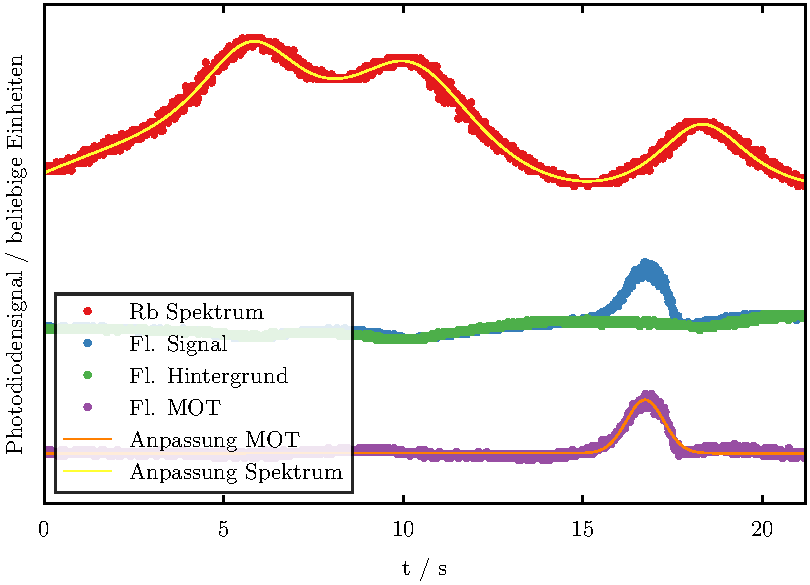
\includegraphics{./figures/detuning_cooling.pdf}
	\caption{Darstellung des Rubidium-Spektrums und der MOT-Fluoreszenz in Abhängigkeit der Verstimmung des Kühllasers. An das Spektrum wurde eine Funktion aus drei Lorentz-Kurven und einem polynomialen Untergrund 4.\ Ordnung angepasst und an das Fluoreszenzsignal der MOT eine Gauß-Kurve.}
	\label{fig:detuning_cooling}
\end{figure}
Im Folgenden soll auf eine Angabe sämtlicher Anpassungsparameter verzichtet werden und nur die Parameter erwähnt werden, die für die weitere Auswertung relevant sind.
Zum einen ist dies die Verstimmung für optimale MOT-Operation, welche aus dem Abstand des Mittelpunkts der Gauß-Kurve (aus der Anpassung an das Fluoreszenzsignal der MOT), zu dem Zentrum der Lorentz-Kurve des Kühlübergangs.
Diese Verstimmung beträgt demnach
\begin{align*}
	\delta = \SI{-11.6 +- 0.4}{MHz} \, \text{,}
\end{align*}
wobei das negative Vorzeichen die erwartete Rotverschiebung signalisiert.
Diese Verstimmung wurde bereits in Abschnitt~\ref{sec:atomzahl} genutzt, um die Anzahl der gefangenen Atome in der Falle zu bestimmen.
Die für den Betrieb einer magneto-optischen Falle optimale Verstimmung~$\delta_\mathrm{opt.}$ ist gegeben durch
\begin{align*}
	\delta_\mathrm{opt.} = -\frac{\Gamma}{2} \, \text{,}
\end{align*}
wobei~$\Gamma$ die natürliche Linienbreite des Kühlübergangs beschreibt \cite{foot}.
Die Linienbreite kann aus der vollen Halbwertsbreite der Lorentz-Kurve an den jeweiligen Übergang gewonnen werden und man erhält aus der Anpassung einer Lorentz-Kurve an den Kühlübergang
\begin{align*}
	\Gamma = \SI{25.7 +- 1.0}{MHz}
\end{align*}
und folglich für die optimale Verstimmung
\begin{align*}
	\delta_\mathrm{opt.} = \SI{-12.8 +- 0.5}{MHz} \, \text{.}
\end{align*}
Man sieht, dass der experimentell bestimmte Wert für die Verstimmung des Kühllasers leicht von dem aus der Theorie erwarteten Wert abweicht.
Dies kann darauf zurückzuführen sein, dass der theoretische Wert~$\delta_\mathrm{opt.}$ nur unter idealisierten Bedingungen gilt, welche in diesem Experiment nicht vollständig erfüllt werden können.


\subsubsection{Variation der Pumplaserfrequenz}
Zuletzt wird die Methode aus den vorigen Abschnitt wiederholt, um den Einfluss der Frequenz des Pumplasers auf die magneto-optische Falle zu untersuchen.
Dazu wird nun der Kühllaser unter einer Rotverstimmung von etwa einer halben Linienbreite auf den Kühlübergang fixiert und der Pumplaser im Scan-Modus unter einer kleinen Scan-Frequenz betrieben.
Die Vorgehensweise zur Entfernung des Untergrundes der Fluoreszenzmessung verbleibt analog zum Abschnitt~\ref{sec:detuning_cooling} und in Abbildung~\ref{fig:detuning_repumping} wurden erneut die Spektren zusammengetragen.
\begin{figure}[h]
	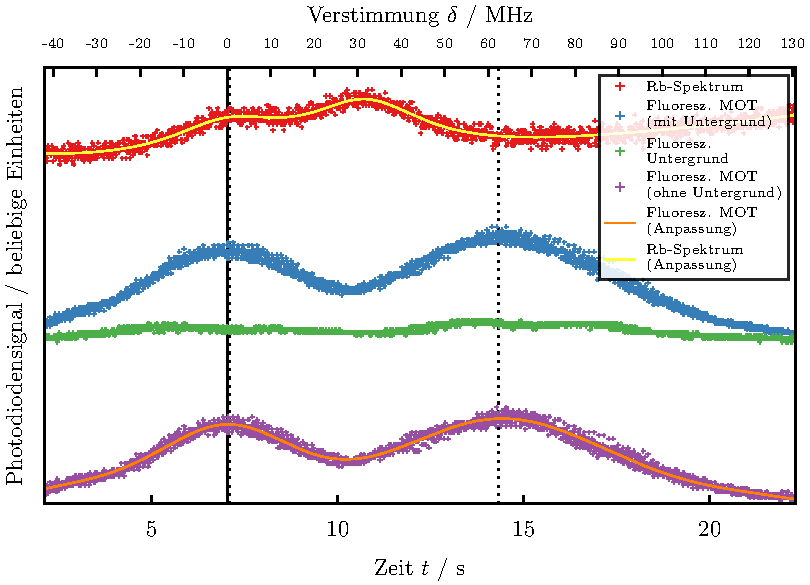
\includegraphics{./figures/detuning_repumping.pdf}
	\caption{Darstellung des Rubidium-Spektrums und der MOT-Fluoreszenz in Abhängigkeit der Verstimmung des Pumplasers. An das Spektrum wurde eine Funktion aus zwei Lorentz-Kurven und einem polynomialen Untergrund 4.\ Ordnung angepasst und an das Fluoreszenzsignal der MOT zwei Gauß-Kurven.}
	\label{fig:detuning_repumping}
\end{figure}

Die Frequenzkalibrierung des Spektrums erfolgt über die beiden Linien im Rb-Spektrum, an welches zwei Lorentz-Kurven mit einem polynomialen Untergrund~4.\ Ordnung angepasst wurde.
Die sichtbaren Linien entsprechen hierbei dem Übergang $F=2 \rightarrow F^\prime=2$ (links) und dem Überkreuzungs-Signal $F=2 \rightarrow F^\prime=2,3$ (rechts).
Zwischen diesen beiden Linien liegt ein Frequenzbereich von \SI{31.7}{MHz} \cite{script}, welcher für die Frequenzkalibrierung genutzt werden kann, um die Frequenzverstimmung zum $F=2 \rightarrow F^\prime=2$ Übergang angeben zu können.
Weiterhin ist anzumerken, dass zwischen die beiden Linien im Rb-Spektrum ein weiteres Überkreuzungs-Signal fällt, welches jedoch nicht klar aufgelöst werden kann.
Darüber hinaus ist der zweite Pumpübergang $F=2 \rightarrow F^\prime=3$ im Spektrum nicht klar zu erkennen, da dieser nur eine kleine Signalhöhe aufweist \cite{script}.

Nachdem die Frequenzkalibrierung erfolgreich war, kann aus der Anpassung von zwei Gauß-Kurven an das gemessene Fluoreszenzspektrum (ohne Untergrund) der jeweilige Linienschwerpunkt und somit die Verstimmung zum $F=2 \rightarrow F^\prime=2$ Übergang bestimmt werden.
Für das linke Maximum im Fluoreszenzspektrum entspricht dies einer Verstimmung von
\begin{align*}
	\delta_{2 \rightarrow 2} &= \SI{0.1 +- 0.5}{MHz}
\end{align*}
und korrespondiert zu einer resonanten Anregung des $F=2 \rightarrow F^\prime=2$ Übergangs.
Dies entspricht den Erwartungen für ein effizientes Pumpen der Rubidium-Atome, welche nach dem Zerfall des angeregten Zustandes erneut in den Kühlkreislauf eintreten können.
Das zweite Maximum der Fluoreszenz zeigt eine Verstimmung von
\begin{align*}
	\delta_{2 \rightarrow 3} &= \SI{62.4 +- 1.4}{MHz}
\end{align*}
und entspricht demnach dem zweiten Pumpübergang $F=2 \rightarrow F^\prime=3$, welcher in \cite{script} mit einer Verstimmung von \SI{63.4}{MHz} zum $F=2 \rightarrow F^\prime=2$ Übergang angegeben ist.
Demnach ist der gemessene Wert für das zweite Fluoreszenzmaximum kompatibel mit einer resonanten Anregung des zweiten Pumpübergangs.

\section{Fazit}

Die Durchführung des Versuchs gelang gut, insbesondere die Justierung der Laser.
Nach kurzer Zeit konnten bereits gefangene Atome beobachtet werden, wobei die Falle durch Veränderungen am Laseraufbau nicht weiter verbessert werden konnte.
Durch Variation und Einstellung der Frequenzen beider Laser konnte die Falle hinsichtlich ihrer Fluoreszenz optimiert werden und eignete sich für die anschließende Charakterisierung.
Der Pumplaser stellte einer Schwierigkeit für die Messungen dar, da er nicht durch eine Rückkopplungsschleife stabilisert werden konnte.
Temperaturdrifts und mögliche andere äußere Einflüsse sorgten dafür, dass sich die Frequenz nach kurzer Zeit bereits so stark veränderte, dass die Fluoreszenzleistung deutlich zurückging und so eine ständige Kontrolle dieser, sowie ein Nachregeln der Laserfrequenz nötig war.

Dennoch konnten aussagekräftige Messwerte aufgenommen werden, die, falls vorhanden, durch Literaturvergleiche als plausibel bewertet werden können. 

\FloatBarrier
% BIBLIOGRAPHIE
\vspace{\fill}
% Maximale Anzahl der Einträge in Klammer
% Zitieren mit \cite{lamport94}
\begin{thebibliography}{19}
\bibitem{anleitung}
	\emph{Advanced Laboratory Course (physics601): Description of Experiments}, BONN-AT-2016-01MP, Universität Bonn, Januar 2016

\bibitem{wieman}
	C.\ Wieman, G.\ Flowers, S.\ Gilbert,
	\emph{Inexpensive laser cooling and trapping experiment for undergraduate laboratories},
	Am.\ J.\ Phys.\ \textbf{63} (4), April 1995.

\bibitem{handbook_spectroscopic_data}
	J.\ E.\ Sansonetti, W.\ C.\ Martin,
	\emph{Handbook of Basic Atomic Spectroscopic Data},
	National Institute of Standards and Technology (NIST), \url{http://physics.nist.gov/PhysRefData/Handbook/Tables/rubidiumtable1.htm} (Letzter Aufruf: 7.\ April 2016).

\bibitem{force_in_mot}
	A.\ M.\ Steane, M.\ Chowdhury, C.\ J.\ Foot,
	\emph{Radiation force in the magneto-optical trap},
	J.\ Opt.\ Soc.\ Am.\ B \textbf{9}, 2142 (1992).

\bibitem{script}
	Skript zum Versuch,
	\emph{FP Experiment: Rubidium MOT},
	(Stand: Januar 2014).

\bibitem{foot}
	C.\ J.\ Foot,
	\emph{Atomic Physics},
	Oxford University Press, 2005.
	
\bibitem{steck}
	D.\ A.\ Steck,
	\emph{Rubidium 85 D Line Data},
	\url{http://steck.us/alkalidata} (Revision 2.1.6, 20.\ September 2013)
\end{thebibliography}

% APPENDIX
\begin{appendix}
\newpage
\section{Anhang}
\end{appendix}

\end{document}
